%%
%% This is file `example/bare_thesis.tex',
%% generated with the docstrip utility.
%%
%% The original source files were:
%%
%% install/buptgraduatethesis.dtx  (with options: `bare-thesis')
%% 
%% This file is a part of the example of BUPTGraduateThesis.
%% 

\documentclass[%
  degree=master,%
  classlevel=open,%
  mathfont=mathptmx,%
  dedication=false,%
  chapbib=false,%
  finish=print,%
  driver=xetex]{buptgraduatethesis}

%% 自定义导言区
%% 在这里添加你需要的宏包、自定义命令、环境等
%% \usepackage{...}
%% \DeclareMathOperator{\CT}{H}
%% \DeclareMathOperator{\Cov}{Cov}
\def\BUPTThesis{\textsc{BUPT}\-\textsc{Thesis}}

%% 在这里添加图片文件搜索目录
\graphicspath{{../}}
%% 自定义导言区结束

%% 加载缩略语定义
%%
%% This is file `example/metadata.tex',
%% generated with the docstrip utility.
%%
%% The original source files were:
%%
%% install/buptgraduatethesis.dtx  (with options: `metadata')
%% 
%% This file is a part of the example of BUPTGraduateThesis.
%% 

%% 涉密论文保密年限
\classdur{三年}

%% 学号
\studentid{2012110191}

%% 论文题目
\ctitle{基于局部特征的图像重建算法研究}
\etitle{Research on image reconstruction algorithm based on local features}

%% 申请学位
\cdegree{工学硕士}

%% 院系名称
\cdepartment{信息与通信工程学院}

%% 专业名称
\cmajor{信号与信息处理}

%% 你的姓名
\cauthor{王继哲}

%% 你导师的姓名
\csupervisor{李学明}

%% 日期自动生成,也可以取消注释下面一行,自行指定日期
\cdate{\CJKdigits{2014}年\CJKnumber{12}月}

%% 中文摘要
\cabstract{%
  中、英文摘要位于声明的次页,摘要应简明表达学位论文的内容要点,体现研究工作的核心思想。
  重点说明本项科研的目的和意义、研究方法、研究成果、结论,注意突出具有创新性的成果和新见解的部分。

  关键词是为文献标引工作而从论文中选取出来的、用以表示全文主题内容信息的术语。
  关键词排列在摘要内容的左下方,具体关键词之间以均匀间隔分开排列,无需其它符号。
}

%% 中文关键词,关键词之间用 \kwsep 分割
\ckeywords{重建 \kwsep 局部特征 \kwsep 图像分割 \kwsep 图像配准 \kwsep 图像融合}

%% 英文摘要
\eabstract{%
  The Chinese and English abstract should appear after the declaration page.
  The abstract should present the core of the research work, especially the purpose and importance of the research, the method adopted, the results, and the conclusion.

  Key words are terms selected for documentation indexing, which should present the main contributions of the thesis.
  Key words are aligned at the bottom left side of the abstract content.
  Key words should be seperated by spaces but not any other symbols.
}

%% 英文关键词,也用 \kwsep 分割
\ekeywords{%
  \TeX \kwsep \LaTeX \kwsep xeCJK \kwsep template \kwsep typesetting \kwsep thesis}


\loadglsentries{acronyms}

%% 攻读学位期间发表论文
%% 用 \newcite{<suffix>}{<caption>} 声明不同的论文类型(例如: 期刊论文、会议论文等)。每一个类型的对应的 .bib 文件用 \bibliography<suffix> 命令加载,用 \nocite<suffix> 命令引用。具体请参考 pubs.tex 中的示例
\newcite{jrnl}{期刊论文}
\newcite{conf}{会议论文}

\begin{document}
%% 声明前置部分
\makefrontmatter

%% 生成主要符号对照表
%%
%% This is file `example/notations.tex',
%% generated with the docstrip utility.
%%
%% The original source files were:
%%
%% install/buptgraduatethesis.dtx  (with options: `notations')
%% 
%% This file is a part of the example of BUPTGraduateThesis.
%% 

\begin{listofnotations}
\item [$(\cdot)^*$] 复共轭
\item [$(\cdot)^{\mathrm T}$] 矩阵转置
\item [$(\cdot)^{\mathrm H}$] 矩阵共轭转置
\item [$\mathbf{X}$] 矩阵或向量
\item [$\mathcal{A}$] 集合
\item [$\mathcal{A}\times\mathcal{B}$]
  集合 $\mathcal{A}$ 与集合 $\mathcal{B}$ 的 Cartesian 积,即 $\mathcal{A}\times\mathcal{B}=\{(a,b):a\in\mathcal{A},b\in\mathcal{B}\}$
\end{listofnotations}


%% 主体部分
\mainmatter
%% 用\include{}命令引用各章.tex文件
%%
%% 第一章 渲染情势
%% 2014.6.25
%% 	http://www.processon.com/#画流程图的软件

\chapter{绪论}
本章主要介绍基于局部特征的图像重建系统在基于云的图像压缩方面的应用场景,该技术的研究背景、国内外的发展情况以及目前取得的研究成果,最后介绍了本文的主要研究内容和文章的组织结构。


\section{论文课题的研究背景}

随着数字化时代的不断发展,智能终端日益普及,终端应用的功能也日趋多样化,我们发现有一类应用服务规模迅速扩大,这一类型的应用采用相似的CS技术架构——智能终端使用传感器采集图像数据,并通过网络向服务器实时传输,由服务器来处理数据,将处理结果反馈给终端用户。而图像应用的爆发式增长给我们带来了一个全新的挑战:图像信息的传输占用了大量的带宽资源。目前的解决方案是在终端对原始图像进行下采样和压缩编码,产生的图像信息的损失大大降低了用户体验,而且传统的压缩编码算法占用了一定的CPU资源,压缩比不是很高,压缩后的图像数据量依然较大。

另一方面,走在大数据时代前沿的互联网拥有无比丰富的图像资源,图像张数数以亿计,图像样式种类五花八门,而且每天还不断有用户贡献着高质量高分辨率的图像。从信息的角度来说,我们拍摄的每一幅图像中所包含的部分或全部内容都可以在互联网上其它图像中找到。

以上两点观察启示我们打破传统的图像内逐像素压缩方法,采用一种全新的基于大数据集的外部图像压缩方法。在2013年6月有学者\cite{Yue:2013gl}提出一种全新的压缩方式——基于云的图像编码。其核心思想是在客户端提取并编码发送少量的图像特征数据,并不传输图像数据本身,而在服务器端解码后利用特征数据在服务器的大图像数据集上匹配相似的图像,利用相似图像进行图像的重建。图\ref{fig:overview}展示了这一客户端-服务器(Client-Service)数据应用模式。
\begin{figure}
\centering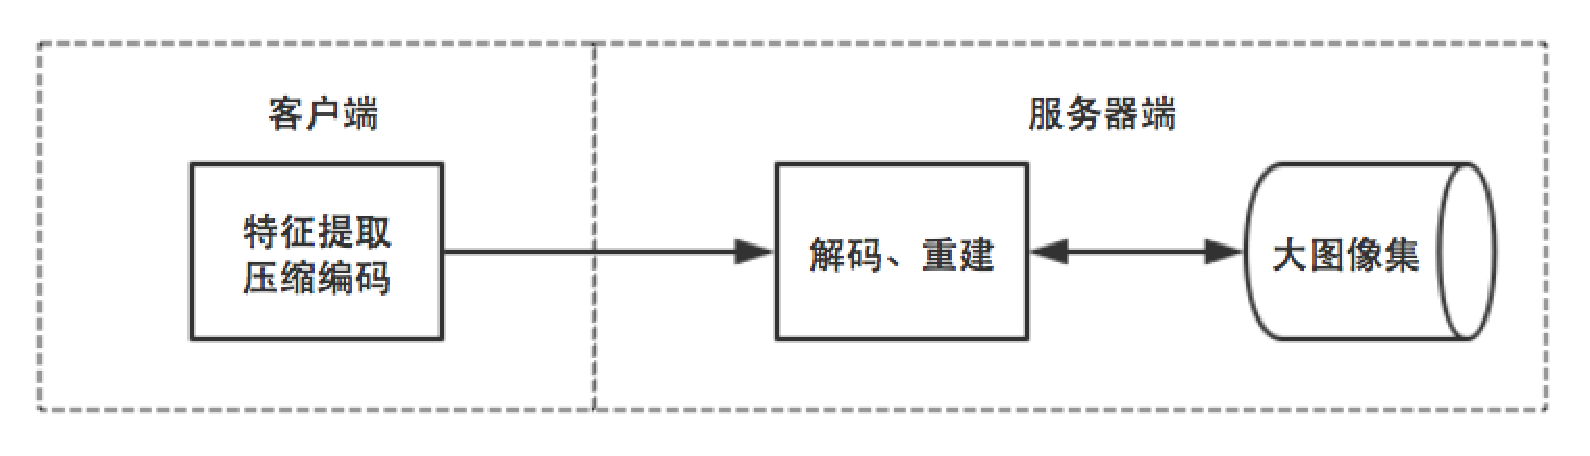
\includegraphics[width=14cm]{imgs/ch1/overview}
\caption{基于与的图像压缩模式}
\label{fig:overview}
\end{figure}
这种架构所运用的核心技术手段便是基于局部特征的图像重建算法,通过对原始图像的特征提取与重建,利用计算资源减少带宽损耗,从一个全新的维度进行数据压缩,为多媒体应用开启了一扇大门。

\section{国内外研究现状}

本文所探讨的基于局部特征的图像重建算法的脱胎于图像拼接技术和相似图像搜索技术,这两个技术相对而言较为成熟:图像拼接领域,SIFT特征的强可区分性和不变性使之广泛应用在全景图拼接领域\cite{Brown:2006ir};相似图像搜索在近年来发展较快,在搜索效率和搜索准确度两个层面进行探索,利用局部特征取代全局特征\cite{Xu:2013wc,POLICY:2013te,Wu:2009bl}以及利用局部特征的空间编码\cite{Zhou:2010tv}进行更为精确的相似图像搜索,使用min-hash等技术对特征进行压缩\cite{Chum:2008jo}提高搜索的速度。

在其上发展而来的基于局部特征的图像重建算法是近几年刚刚提出的一项新颖的技术手段,Philippe Weinzaepfel等人于2011年首先提出了基于局部特征进行图像的重建\cite{Weinzaepfel:2011jh},重建方法首先是根据局部特征使用传统技术在大数据集上找到与原始图像视觉相似的图像块,通过特征匹配与配准将候选图像块转换到标准图像域,通过无缝拼接技术将其拼合在一起,最后使用平滑差值计算空白区域的像素值,以椭圆形图像块为基本单元,重建的结果如图\ref{fig:Weinzaepfel_res}所示。

\begin{figure}
\centering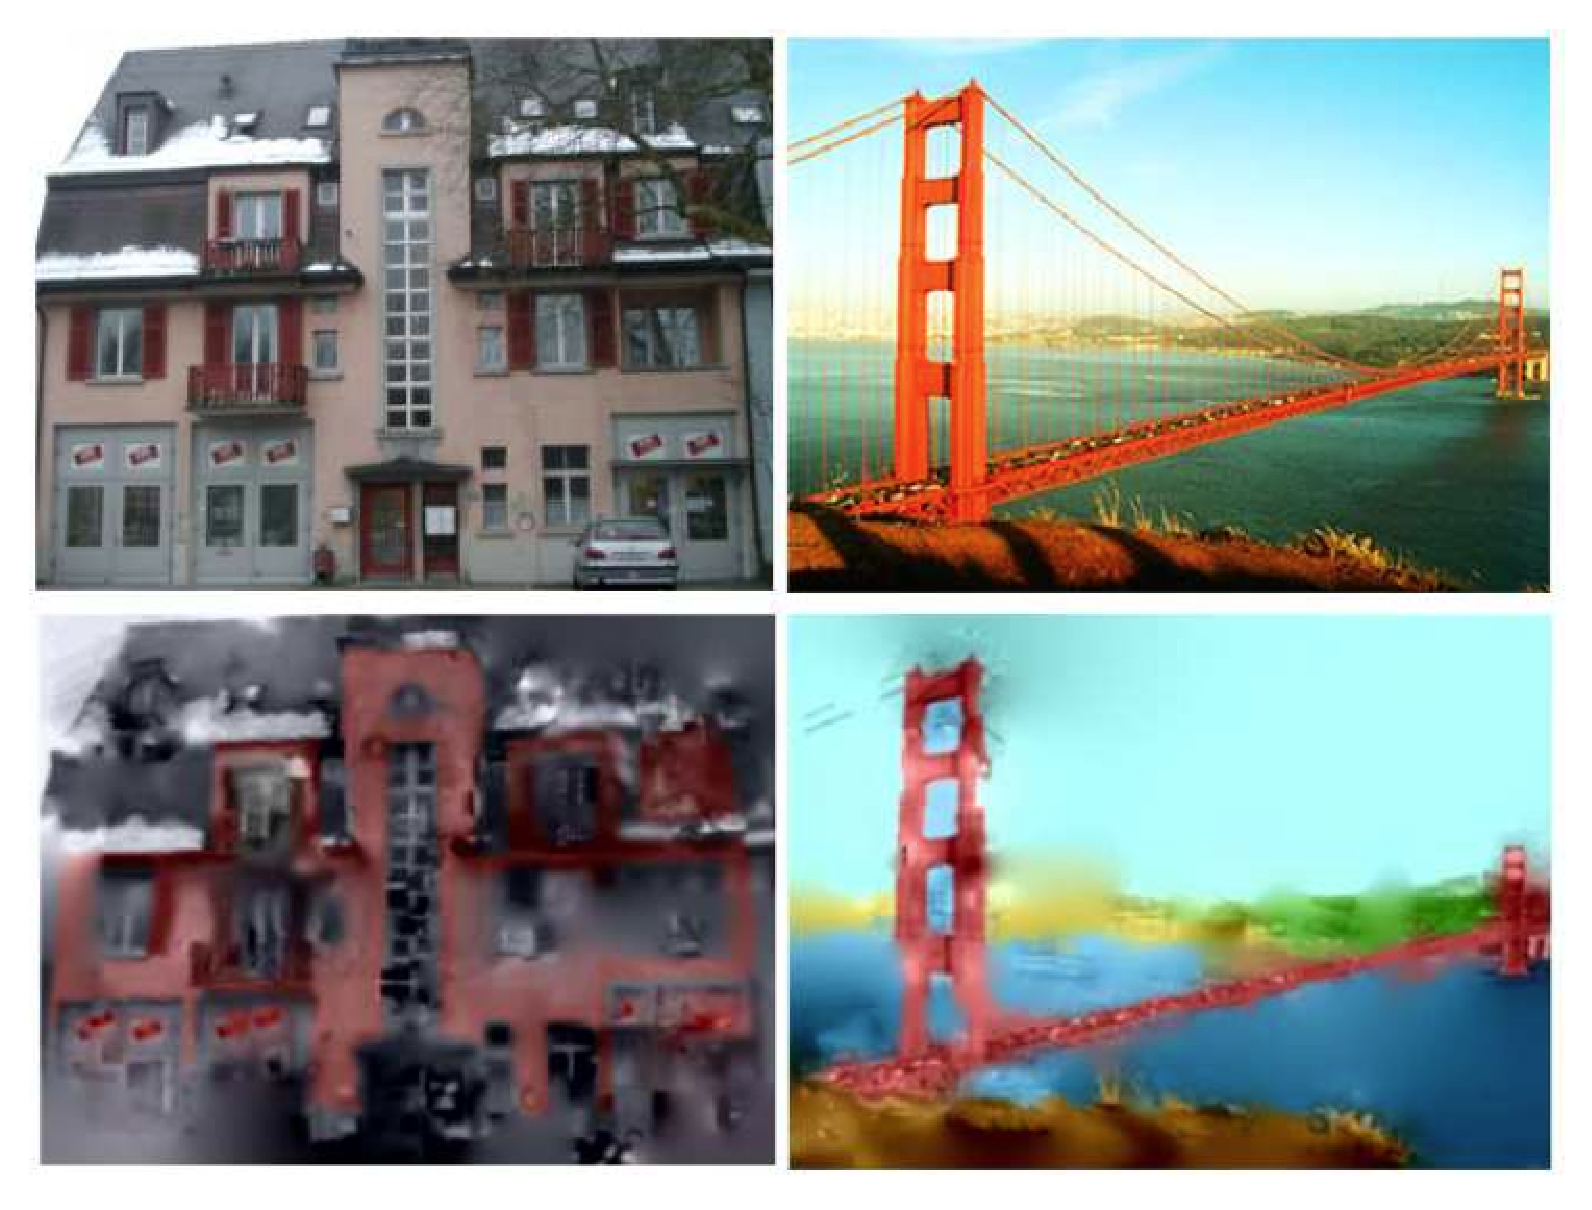
\includegraphics[width=15cm]{imgs/ch1/Daneshi_res}
\caption{Daneshi基于局部特征的图像重建结果}
\label{fig:Daneshi_res}
\end{figure}

在这一自动化的图像重建系统中,虽然重建结果没有达到视觉满意程度,但是显示了基于特征进行重建的可能性,作者由此提出了图像的局部特征信息可能泄露用户隐私这一话题。

随后,Maryam Daneshi和Jiaqi Guo\cite{Daneshi:2011wi}则在确实特征尺度信息的前提下,挖掘图像重建的最大可能。他们采用方形图像块作为重建的基本单元,利用贪婪算法逐步的学习每一个图像块的尺度,完成图像的亮度信息重建,最后采用用户指定颜色遮罩并用最优化算法来进行上色,重建结果如图\ref{fig:Daneshi_res}所示,重建结果保留了大部分的图像信息。

\begin{figure}
\centering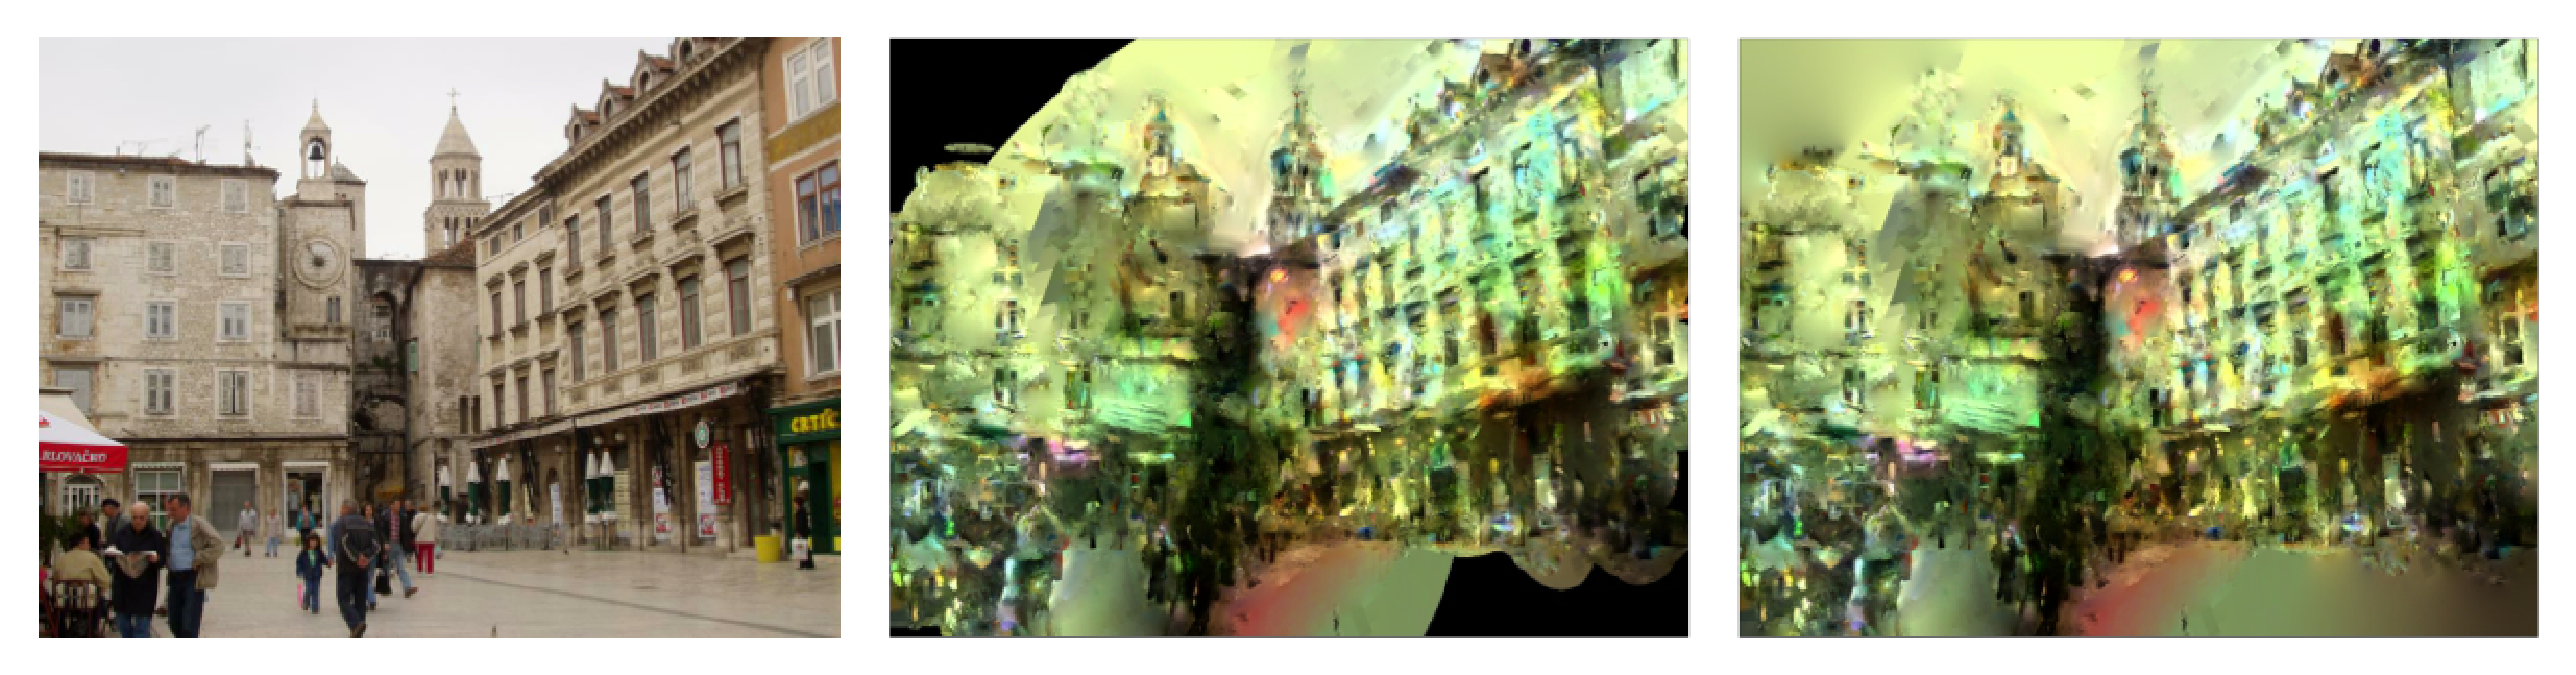
\includegraphics[width=15cm]{imgs/ch1/Weinzaepfel_res}
\caption{Weinzaepfel基于局部特征的图像重建结果,从左向右依次是原始图像、重建图像、补全后的图像}
\label{fig:Weinzaepfel_res}
\end{figure}

Lican Dai等人提出将其应用在手机地标图像的实时分享\cite{Dai:2012vn},采用基于搜索的重建技术搭建了IMShare系统,提出使用缩略图来指导服务器端的特征提取和图像融合,实验结果显示缩略图的使用大大提升了图像的重建结果,该系统不仅能够重建人眼视觉满意的图像,而且采用并行的处理手段,能在秒这一数量级上完成重建流程。Huanjing Yue使用相似的技术手段进行超分辨率的图像生成,使用低分辨率(LR)的图像在大数据集上进行搜索,得到高分辨率(HR)的候选图像,再通过特征提配与图像重建的技术手段生成超分辨率图像(SR)。

综上所述,基于局部特征的图像重建算法是一项较新的领域,将其用在图像在客户端和服务器端压缩传输更是一个全新的领域,有着大量的技术难点需要攻克,本文主要是在这一应用场景下,对其中的各种技术手段做进一步的探索。

\section{论文的主要研究内容与章节安排}
\subsection{主要研究内容}

本课题以文献\cite{Yue:2013gl}提出的核心任务与技术框架为基础,重点研究在基于云的图像压缩应用场景下的基于局部特征的图像重建算法,进一步探索利用更丰富的图像特征信息在大语料集中进行高质量的图像重建,使重建图像质量达到人眼主观效果较好的程度。重建任务的核心是通过局部特征找到与原始图像相似的图像单元以及可靠的图像间对应点集合,进而自动地建立图像之间点与点或区域与区域之间的可靠对应关系,根据对应关系采用一定的算法拼接图像单元。基于局部特征对图像进行重建的技术能够让我们在发送端只传输少量的特征数据,而接收端服务器利用大数据集进行高分辨率图像的还原。文献\cite{Yue:2013gl}创新性的提出了基于云的图像编码方式,核心思想是以客户端进行特征提取,在服务器端利用局部特征在大规模图像集上找到相匹配的图像块,利用计算机视觉相关算法将图像块拼合成一幅完整图像,达到图像重建的目的,其服务体系如图\ref{fig:service}所示。

\begin{figure}
\centering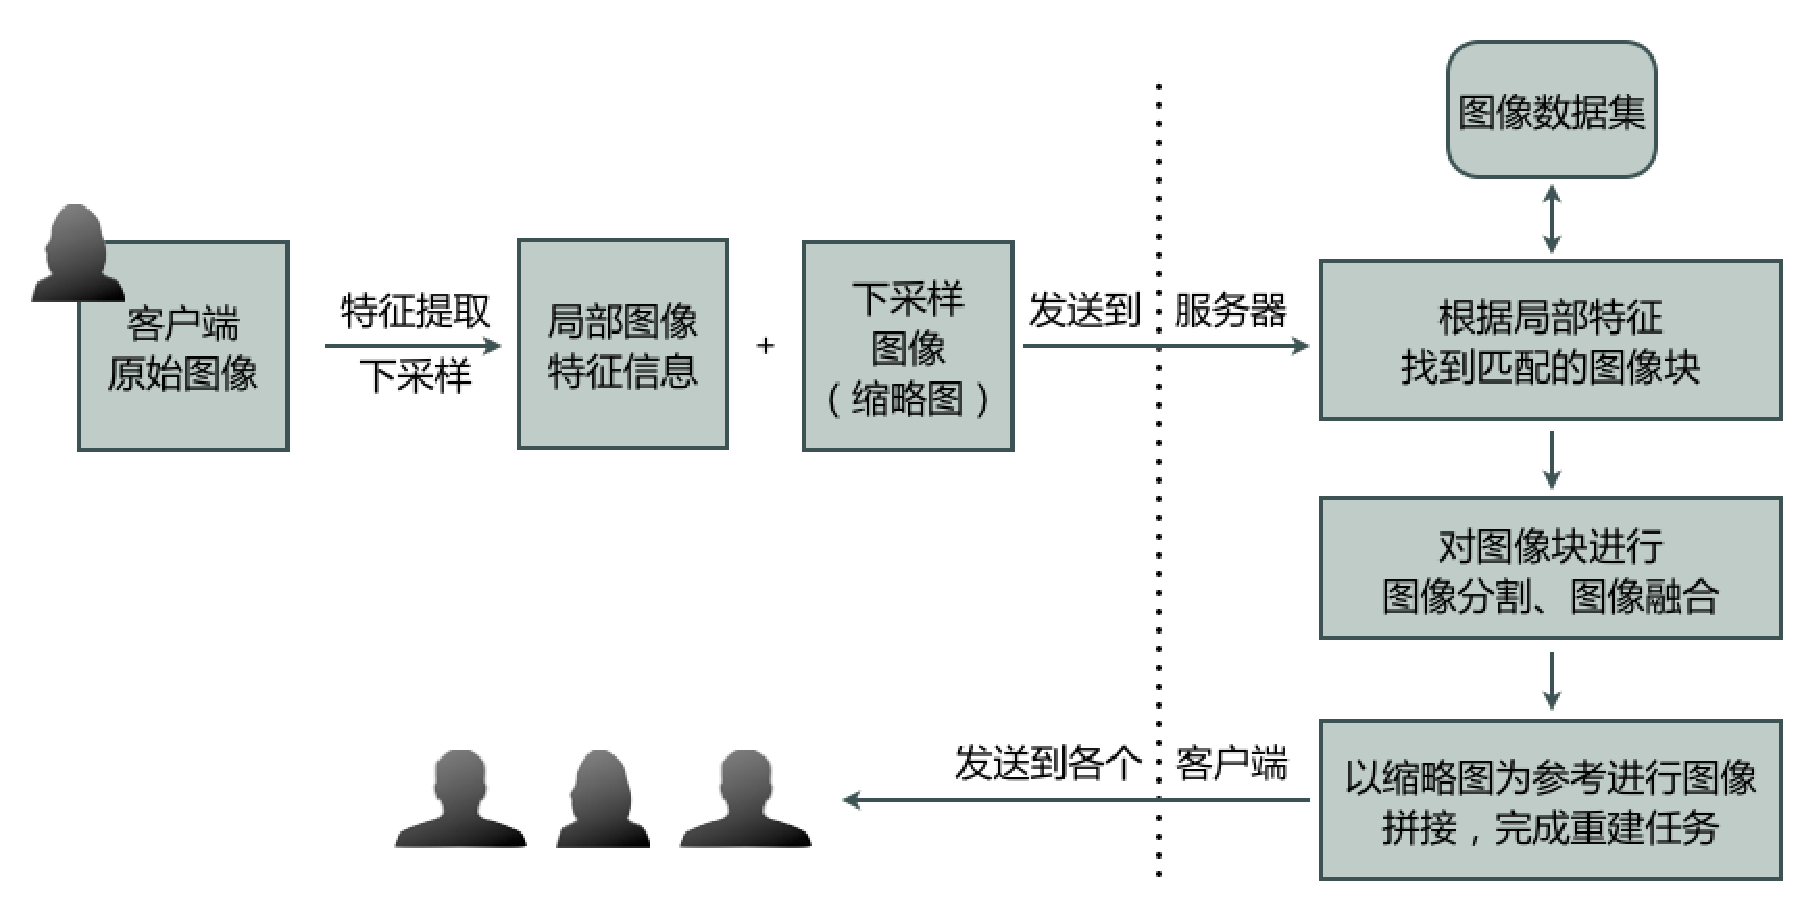
\includegraphics[width=15cm]{imgs/ch1/service}
\caption{基于云压缩的图像服务}
\label{fig:service}
\end{figure}

它主要解决的是在当前手机网络带宽有限的情况下图像的实时分享问题,我国大部分区域还是在2G和3G网络覆盖下,传输一张高分辨率的JPEG图像需要几分钟的时间。并且处理的过程需要占用大量的手机资源,传输的延时和图像分辨率的压缩带来不佳的用户体验。为了解决上述难题,作者提出了基于云压缩的方式进行图像传输:在手机端,下采样获取手机图像的缩略图,使用特征检测与特征描述获取SIFT特征。利用缩略图压缩SIFT算子,经过压缩后,每幅图像能够保持在10KB左右的大小,大大加快了传输速度;在云端有一个大图像数据集,可以通过特征描述借用数据集进行图像的重建;最终,重建的结果以不同分辨率的形式分发到其他用户终端上。

本文在上述的大框架下综合使用多种信息检索与图像处理技术,使用了上述系统中相同的数据编解码方式,而对其中的相似图像检索、图像块筛选等核心算法进行了改进与完善,使之更加能够适用于大规模图像集上的图像重建任务,重建结果得到了进一步的优化。

因此,课题将深入研究基于局部特征进行图像重建任务中的各个环节。从技术范畴来说,本课题可以归纳为两个方面:

\begin{enumerate}
\item 一方面是在计算机视觉领域综合运用图像关键点的提取、局部特征描述、特征匹配、图像配准、图像分割、图像融合等图像处理算法,形成一套完整的基于局部特征进行图像重建的算法流程;
\item 另一方面是针对大数据集的处理,由于图像的匹配与重建等相关任务是建立在大数据集基础之上的,所以本课题试图探索如何在大规模图像集上优化现有的图像重建方案,拟采用改进的聚类算法生成视觉词,利用k-d树等数据结构组织视觉词并进行快速的词条匹配,探索重建任务的并行解决方案。
\end{enumerate}


\subsection{章节安排}
本文分为五个章节,具体内容为:

第一章 绪论。综合论述了立题的意义、背景和课题价值,基于局部特征的数字图像重建算法国内外的研究现状及进展,并进行了归纳,提出了本文研究的应用场景及相关技术,最后总结了本文的章节结构。

第二章 系统概述。主要介绍图像重建算法在基于云的压缩这一场景下的使用。着重介绍本文的系统整体框架,各个模块的输入输出与所使用的技术和算法。

第三章 基于局部特征的图像重建算法。三、四章从两大主要技术环节出发,深入探讨系统所使用的具体算法。第三张从传统的局部特征着手,探讨了图像的匹配、配准、融合等技术手段,并针对大语料集的重建任务对上述算法做了优化与完善。

第四章 大规模近似重复图像搜索算法。探讨系统中所使用的相似图像搜索技术,探讨了从传统的全局特征搜索到局部特征搜索的的发展状况,分析了近期局部特征的使用在相似图像搜索领域的新的发展,从算法的搜索效率与搜索结果多样化两方面对算法进行优化。

第五章 总结与展望。本章总结了目前的工作成果,并对今后基于局部特征的相似图像搜索的研究方向进行了探讨。

%% 本章参考文献
\ifx\usechapbib\empty
\nocite{BSTcontrol}
\bibliographystyle{buptgraduatethesis}
\bibliography{bare_thesis}
\fi

%%
%% 第二章
%% 2012.5.20

\chapter{基于相似图像集的图像重建算法}

从重建流程划分,重建算法(1)首先使用请求图像的局部特征在大数据集上进行相似图像的搜索,将搜索结果中最为相似的若干张图像作为重建候选图像集;(2)利用请求图像的局部特征在候选图像集上做更为精确的图像重建。本文按照以上两个技术层面分别进行阐述,本章探讨如何使用小规模候选图像集进行图像重建及其优化策略,下一章着重探讨大规模图像搜索领域中的相似图像搜索算法。

% 图像重建可以被概括的定义为这样一个基本问题:从一个退化版本的二维物体估算实际的二维物体\cite{Demoment:1989tw}。退化过程的数学形式取决于图像重建算法实际的应用场景。

% %%%%---------------------------------------传统的图像重建算法---------------------------------------------%%%%
% \section{传统的图像重建算法}
% 传统的图像图像重建算法所使用的场景一般是指图像修复(Image Restoration),原始“物体”由于经历了某种退化过程,不能直接由观测信息判断出来,为了消除退化过程的影响,必须根据观测到的数据进行重建来还原得到原始信息。
% 在图像修复中,引起退化的原因叫做失真,其定义如下:
% \begin{equation}
% y = A(X) \bullet b
% \end{equation}
% 其中\(A(\cdot)\)是退化函数,可以看做是一个滤波器,b表示的是噪声,\(\bullet\)表示的叠加方式。失真通常包含对X的卷积或者模糊,加性噪声或者乘性噪声。
% 而图像修复的解决方案是通过对观测信息进行退化模型的数学建模,利用约束条件来推导出退化过程的逆过程,对观测信息进行逆过程得到原始图像。

% 另一类图像重建场景是超分辨率重建,在近年来得到飞速的发展,是炙手可热的研究领域,它的基本思想是通过多张连续的低分辨率图像序列得到一张高分辨率的图像。很多数字图像应用中都需要高分辨率的图像,高分辨率的图像能够提供更佳的视觉体验,提供更丰富的信息,比如高分辨率的医学图像能够让医生更好的进行病情诊断,高分辨率的卫星图像能够进行更准确的模式识别任务。从1970年代以来,CCD和CMOS传感器被大规模的使用,获得了大量的数字图像,但是很多图像的分辨率较低,不能满足日益增长的业务需求,超分辨率重建是在这样的背景下诞生的\cite{Park:2003hg}。

% 那么,我们如何通过多张低分辨率图像获得一个高分辨率图像呢?如果一个场景下有多张低分辨率图像,而且这些图像从不同的角度来“描述”这个场景,那么这些低分辨率的图像可以看做是该场景的子采样和子像素精度的位移。如果这些低分辨率图像是以整数像素为单位进行的位移,那么多张低分辨率图像没有提供任何“新的信息”,但是如果位移单位是子像素单位的,序列中的每一个图像不能够由其他图像得出,换言之每个图像都提供了子像素精度的不同信息,我们可以利用这些信息重建一个高分辨率的图像。
% 一般来说,SRR算法分为基于重建和基于学习的两大类:基于重建的算法如频域重建法利用图像序列的交叠关系,凸集投影(POCS)等利用一些先验知识来约束求解过程,以达到增加细节信息的目的;基于学习的算法则使用多种机器学习的概率模型,包括基于流形学习、基于支持向量机和基于独立分量的超分辨率重建技术。基于学习的方法采用大量的高分辨率图像构造学习库来训练学习模型,在对低分辨率图像进行重建的过程中引入由学习模型获得的先验知识,进而得到图像的高频细节,获得较好的图像重建效果。

% 总体而言,超分辨率重建的整个流程包括三个基本环节:
% (1)低分辨图像的预处理,包括降噪和裁剪等基本图像数据处理。
% (2)配准过程,利用像素的空间信息估算低分辨率序列图像之间的运动矢量和空间位置关系。
% (3)完成重建,使用图像分割和融合等技术,利用多帧低分辨率图像的信息完成超分辨率重建。
%%%%-------------------------------------于局部特征的图像重建算法---------------------------------------------%%%%

本文所采用的图像重建的部分流程可以看成是多幅图像的全景图拼接问题。与文献\cite{Brown:2006ir}中的流程类似,主要包含以下几个环节:(1)使用具有不变性的特征来描述图像;(2)自动的找到图像之间的空间位置关系,进行图像配准;(3)图像融合,消除不同图像之间的光照差别,去除边缘噪声。与全景图拼接不同的是,本文使用的图像重建算法以图像块(Patch)作为拼接的最小单位,图像块像素数量分布不均匀、图像块之间有大量的重叠区域、图像块位置不够精确等特征点给拼接带来了一定的难度。本章从上述技术环节出发,分别探讨图像局部特征、特征匹配、图像配准等环节,并提出了针对图像块拼接的优化方案。

%%%%----------------------------------------局部特征---------------------------------------------%%%%
\section{图像的局部特征}

\subsection{局部特征概述}
图像的局部特征是计算机视觉领域一个基本问题,它能够反映图像某一局部的特性,对寻找图像对应的局部单元以及特征描述有着重要作用。通常意义的局部特征包含两个方面,特征检测子(Detector)和特征描述子(Descriptor)。检测子能够检测出我们“感兴趣”的点或者局部区域,而一个好的局部特征描述子反映出图像的局部特性能够帮助找到图像与图像点集合对应关系,进而建立图像之间的空间对应关系。局部图像特征描述的核心问题是不变性(invariant)和可区分性(discrimination)。

\begin{enumerate}
\item 不变性:指的同一局部特征经过不同的变换之后,仍然具有较强的相同特性,例如光照或透视产生变换后,同一描述子仍然能够被识别。
\item 可区分性:指的是描述不同局部特征的描述子有着较大的差别,可以被显著的区分。
\end{enumerate}

然而特征描述子的可区分性的强弱和其不变性是矛盾的,也就是说,一个具有诸多不变性的特征描述子,它区分图像局部内容的能力就稍弱;而一个非常容易区分不同图像局部内容的特征描述子,它的鲁棒性往往比较低。因此,在基于局部特征的图像处理中,研究不仅具有较强不变性、还具有较好区分性的特征描述子有着重要意义。

目前人们提出的众多图像局部特征算子中,由Lowe提出的尺度不变特征变换(Scale Invariant Feature Transform,简称SIFT)应用最为广泛。1999年首次提出,至2004年得到完善\cite{Lowe:2004uq}的SIFT算子是图像局部特征研究领域的一项重大突破。SIFT算子具有很强的可区分性,同时对尺度、旋转以及一定视角和光照变化等图像变化都具有不变性。在其之上衍生出来的SURF(Speeded Up Robust Features)是对SIFT的改进版本,它利用Haar小波来近似SIFT方法中的梯度操作,同时利用积分图技术进行快速计算,SURF的速度是SIFT的3-7倍。

除此以外,常见的特征检测子包括Harris角点,ANMS等,描述子还包括DAISY,ASIFT,MROGH,BRIEF等,分别适用于不同的图像应用场景下,本文提出的系统采用适用性最广泛的SIFT算子,下面我们对其进行简要的介绍。

\subsection{尺度不变特征变换}

(1)尺度空间理论

尺度空间理论目的是模拟图像数据的多尺度特征。尺度空间中各尺度图像的模糊程度逐渐变大,能够模拟人在距离目标由近到远时目标在视网膜上的形成过程。我们可以把两幅图像想象成是连续的,分别以它们作为底面作四棱锥,就像金字塔,那么每一个截面与原图像相似,那么两个金字塔中必然会有包含大小一致的物体的无穷个截面,但应用只能是离散的值,所以我们只能构造有限层,层数越多步长越小,特征描述越精确,但处理时间会相应增加;层数太少不行,因为向下采样的截面中可能找不到尺寸大小一致的两个物体的图像。一个图像的尺度空间\(L(x,y,\sigma)\)定义为一个变化尺度的高斯函数\(G(x,y,\sigma)\)与原图像\(I(x,y)\)的卷积。
\begin{equation}
  L(x,y,\sigma) = G(x,y,\sigma) \otimes I(x,y)
\end{equation}

图\ref{fig:DoG}反映了图像金字塔的情况:

\begin{figure}
\centering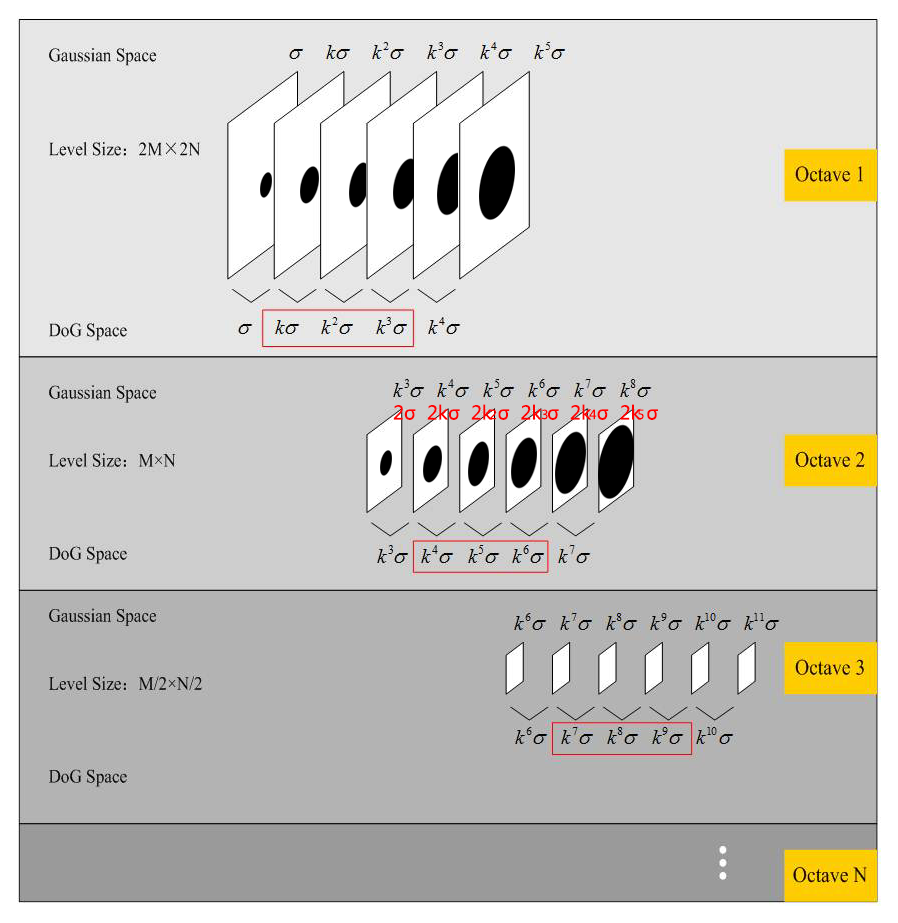
\includegraphics[width=15cm]{imgs/ch2/DoG}
\caption{尺度空间与金字塔模型}
\label{fig:DoG}
\end{figure}

图中的黑色圆盘表示的是该图像所在的尺度的特征覆盖的范围,其特点是不同组同一层上的特征覆盖范围一样,同一组不同层上的特征覆盖范围逐步增大。关键点的尺度坐标就是按关键点所在的组和组内的层,利用下面这个公式计算而来:
\begin{equation}
  \sigma(o,s) = \sigma_0 2^{o+s/S},
  \quad o \in o_{\min} + [0, ..., O-1],
  \quad s \in [0,...,S-1]
\end{equation}

(2)SIFT检测子

SIFT算法有两个主要环节,一个是检测“感兴趣”的关键点,另一个是描述这个“关键点”。SIFT关键点是精心选择的一组在高斯差分尺度空间(Difference of Gaussians scale space,DoG)上的极值点,该关键点包含三个关键信息,分别是(1)亚像素精度的(x,y)位置信息;(2)尺度大小,反映关键点在局部的影响范围,决定了特征的覆盖区域像素数量,对后文局部图像块的提取起到至关重要的作用;(3)所在高斯尺度空间上的主方向,该主方向是有一个高斯窗口函数计算得来,反映的是关键点所在局部的方向信息。其中差分高斯尺度空间表示为
\begin{equation}
  D(x,\sigma(s,o)) \doteq G(x,\sigma(s+1,o)) - G(x,\sigma(s,o)).
\end{equation}

关于尺度空间和描述子的具体讲解在Lowe的论文中\cite{Lowe:2004uq}已有详细的介绍,这里不再详述。

(3)SIFT描述子
SIFT描述子反映关键点局部的信息,是高斯尺度空间上某一局部和方向上的梯度信息,以直方图的形式对信息做统计,最终每一个描述子是一个128的特征。

%%%%----------------------------------------匹配--------------------------------------------%%%%
\section{特征匹配}
提取图像的局部特征之后,我们希望找到两幅相似的图像间相一致的特征点,这一过程叫做特征匹配。匹配环节最重要的两个步骤是匹配策略的确定和高效的数据结构以及相应的匹配算法。

\subsection{匹配策略}
如果我们知道一个SIFT描述子和其它所有描述子的相似程度的数值表示,就可以采取如下的匹配策略:
\begin{equation}
  M(S,S_r) = 
\begin{cases} 
\text{true}, & \mbox{if } S_r = S_{min},\frac{\text{Dis}(S,S_{min})}{\text{Dis}(S,\tilde{S}_{min})} > C \\
\text{false}, & \mbox{otherwise}
\end{cases}
\end{equation}

\(S\)是我们待匹配的描述子,\(S_r\)是所有候选描述子中的一个,\(S_r = S_{min}\)说明\(S_r\)是与待匹配描述子最为接近的一个。\(\text{Dis}(\cdot,\cdot)\)表示的是两个特征描述子之间的相似性度量,比如可以用欧氏距离表示,距离越大,相似性越小。\(S_{min}\)和\(\tilde{S}_{min}\)分别表示的是与S距离最近和第二近的特征。而C是一个阈值常数,通常取1.5。上式表明,如果最匹配的特征的距离比其次匹配特征的距离的比值大于一定的程度,我们认为该特征有最佳匹配,最佳匹配就是最为相似的特征;如果比值小于阈值,则认为匹配失败。

\subsection{高效匹配算法}
在上述的匹配策略中,我们有这样一个前提,能够比较当前特征点和每一个候选特征点的相似性,进而找到最为相似的一个候选特征。在解决这个最近邻问题时,总体的时间复杂度是\(O(n^2)\),在大多数的应用中使用并不现实。因此我们需要找到更为合适的索引结构来存储数据,进行快速的查找。解决这种高维数据查询检索的一些常见算法包括使用多维散列,局部敏感哈希(Locality Sensitive Hashing)以及多维搜索树等。本文使用多维搜索树中最为常见的k-d树(K-dimension tree),下面对其做简要介绍。

k-d树是一种空间划分树,它把整个特征空间交替沿着垂直于坐标轴的超平面将空间进行分割,分割时尽量使得特征点的分布保持平衡。然后在特定的划分内进行相关搜索操作,有效减少搜索范围。

构建k-d树遵循如下的规则:

(1)随着树的深度增加,循环的选取坐标轴,作为分割超平面的法向量。对于维度为3的树来说来说,根节点选取x轴,根节点的孩子选取y轴,根节点的孙子选取z轴,根节点的曾孙子选取x轴,这样循环下去。

(2)每次均为所有对应实例的中位数的实例作为切分点,切分点作为父节点,左右两侧为划分的作为左右两子树。

对于n个实例的k维数据来说,建立k-d树的时间复杂度为O(k*n*logn)。

k-d树的搜索算法如下\cite{李航2012统计学习方法}:
\begin{enumerate}
\item 在k-d树种找出包含目标点x的叶子节点:从根节点出发,递归访问k-d树。若x当前维的坐标小于切分点的坐标,则移动到左子结点,否则移动到右子节点。直到叶子节点。
\item 以当前叶子节点为“当前最近点”。
\item 回溯:递归的回退,对每个节点:

	\begin{itemize}
	\item 如果该节点比当前最近节点离目标更近,则更新“当前最近点”
	\item 当前最近点一定存在于该节点某个子节点对应的区域,检查该子节点的兄弟节点对应的区域是否有更近的点。
	\end{itemize}

\item 回退到根节点,结束,“当前最近点”即为我们找到的最近邻。
\end{enumerate}
%%%%----------------------------------------配准--------------------------------------------%%%%
\section{图像配准}

在得到两幅图像(在本文中是两个图像块)相匹配的特征点之后,我们有了相对应点的位置关系,如何利用这些位置关系将两幅图像重合的部分放置于正确的位置上,是本节讨论的议题。

\subsection{直接变换法}
我们可以根据两个图像块的位置、方向、尺度直接写出两个图像块之间的变换公式,我们称作直接法,本节首先介绍各种2D变换,最后介绍如何根据匹配图像块的空间信息直接写出变换矩阵。

(1)旋转和平移变换,也叫2D刚体运动即2D欧式变换(因其保持欧式距离),写作\(x={Rx+t}\)或者写作
\begin{equation}
	\begin{bmatrix}
	R & t
	\end{bmatrix}
	\bar{x}
\end{equation}
其中
\begin{equation}
	\begin{bmatrix}
	\cos{\theta} & -\sin{\theta} \\
	\sin{\theta} & \cos{\theta}
	\end{bmatrix}
\end{equation}
是一个正交旋转矩阵,有\(RR^T = I\)和\(|R| = 1\)

(2)放缩旋转,也叫做相似变换,该变换可以表示为\({\bar{x}}={sRx+t}\),其中s是一个任意的尺度因子。它也可以写作
\begin{equation}
	x ={ 
	\begin{bmatrix}
	sR & t
	\end{bmatrix}
	\bar{x}
	}
	={
	\begin{bmatrix}
	a & -b & t_x \\
	b & a & t_y
	\end{bmatrix}
	\bar{x}
	}
\end{equation}
其中我们不再需要\(a^2 + b^2 = 1\)。相似变换保持直线间的夹角。
各种2D变换如表\ref{2dtrans}所示。

\begin{table}[h]
\caption{2D坐标变换}
\label{2dtrans}
\centering
\begin{tabular}{|c|c|c|c|}
\hline
\textbf{变换} & \textbf{矩阵大小} & \textbf{自由度数} & \textbf{保持} \\ \hline
平移          &   \(2\times{3}\)	& 2             & 方向          \\ \hline
刚性(欧式)    &   \(2\times{3}\) & 3             & 长度          \\ \hline
相似          &   \(2\times{3}\)  & 4             & 夹角          \\ \hline
仿射          &   \(2\times{3}\)  & 6             & 平行性         \\ \hline
投影          &   \(2\times{3}\)   & 8             & 直线性         \\ \hline
\end{tabular}
\end{table}


当我们使用SIFT算法得到匹配到的特征点后,可以根据一对匹配的SIFT算子直接写出两个图像块的变换矩阵,我们称这个变换为\(H_0\),具体求解方式如下:

结合一对匹配SIFT特征点\(\tilde{S}\)和\(S\)的位置、尺度和方向,我们可以得到两个图像块\(P_{\tilde{S}}\)和\(P_S\)的变换矩阵\(H_0\):

\begin{equation}
	H_0 = 
	\begin{bmatrix}
	\frac{\tilde{s}_f}{s_f} R & T
	\end{bmatrix}
\end{equation}
其中
\begin{equation}
	R = 
	\begin{bmatrix}
		\cos{(\tilde{\theta}-\theta)} & -\sin{(\tilde{\theta}-\theta)} \\
		\sin{(\tilde{\theta}-\theta)} & \cos{(\tilde{\theta}-\theta)} 
	\end{bmatrix}
\end{equation}

\begin{equation}
	T = 
	\begin{bmatrix}
		\tilde{x}_f - x_f \\
		\tilde{y}_f - y_f
	\end{bmatrix}
\end{equation}

下面我们介绍如何使用随机抽样一致算法求解\(H\)。

\subsection{随机抽样一致算法}
随机抽样一致(RANdom SAmple Consensus,RANSAC)是一种空间匹配算法。该算法将数据分成两类,局内点(inlier)和局外点(outlier)它可以从一组包含局外点的观测数据集中,通过迭代方式估计数学模型的参数。

这是一种不确定的算法,有一定的概率得出一个正确的或者说是可接受的合理结果;一般情况下,迭代次数的增加可以提升结果的准确性。该算法由Fischler和Bolles于1981年提出,在图像检索中,RANSAC可以作为检索后的后续处理,对图像中的目标进行空间一致验证。

RANSAC算法对数据集做了三个假设:

\begin{enumerate}
\item 数据由局内点组成,局内点的数据的分布符合某一特定的概率模型;
\item 与局内点相对的是局外点,他们不能够适应该模型;
\item 局内点与局外点之外的数据属于噪声
\end{enumerate}

RANSAC有以下几个步骤:
\begin{enumerate}
\item 随机选择数据集合的一个子集;
\item 使用所选择选择的子集拟合出一个数学模型,在;
\item 确定该模型下局外点的个数;
\item 重复步骤1~3若干次,以最好的一次结果最为最终拟合出来的数学模型。
\end{enumerate}

RANSAC算法迭代次数的选取取决于我们期望的准确率与样本数量。设p为任意给定对应点合法的概率,即
\[p = \frac{\text{局内点的数量}}{\text{数据集全部数据的数量}}\]
而P是经过S次试验后成功的总体概率。设我们需要k个随机样本来估计模型,那么在一次试验中,该k个样本都是局内点的可能性为\(p^k\)。因此,S次试验失败的可能性是
\[1 - P = (1 - p^k)^S\]
两边去对数,得到最少需要的试验次数是
\[S = \frac{log(1-P)}{log(1-p^k)}\]
随着k的增大,需要的最少试验次数增多,在实际中,我们应该尽可能的选择小的k值。在模型确定以及最大迭代次数允许的情况下,RANSAC总是能找到最优解。对于含有较大误差的数据集,RANSAC的效果远优于直接的最小二乘法。

当对两幅图像进行匹配的时候,所以相互匹配的局部特征作为数据全集,我们要估算的模型是一个变换矩阵H,能够将图像\(I\)投影到图像\(I'\)。每次迭代过程中,随机的选择四对匹配的特征点,根据这四个特征点的位置信息解得变换H,利用H计算其它匹配对的位置信息中有哪些属于局外点,记录局外点的个数。局外点的个数越少,变换矩阵H越准确。反复迭代多次得到一个相对准确的透视变换模型。

上述提到的用四对匹配点拟合出的变换矩阵叫做单应矩阵(Homography),最简单的求解单应性矩阵的算法叫做直接线性变换法(Direct Linear Transform,DLT)\cite{Dubrofsky:2009tz},其具体算法如下:

假设我们相匹配的一对点分别是\(x\)和\(x'\),单应性矩阵是\(H\),那么有如下等式:

\begin{equation}
\label{homography1}
	c
	\begin{pmatrix}
	u \\
	v \\
	1
	\end{pmatrix}
	= H
	\begin{pmatrix}
	x \\
	y \\
	1
	\end{pmatrix}
\end{equation}


其中c是一个非零常数,\((u\ v\ 1)^\mathrm{T}\)代表\(x'\),\((x \ y \ 1)^\mathrm{T}\)代表\(x\),而
\(
H = 
\begin{pmatrix}
h_1 & h_2 & h_3 \\
h_4 & h_5 & h_6 \\
h_7 & h_8 & h_9
\end{pmatrix}
\)

将公式\eqref{homography1}展开,分别用第一行和第二行除以第三行,得到

\begin{equation}
\label{homography2}
-h_1x - h_2y - h_3 + (h_7x+h_8y+h_9)u = 0
\end{equation}

\begin{equation}
\label{homography3}
-h_4x - h_5y - h_6 + (h_7x+h_8y+h_9)u = 0
\end{equation}

公式\eqref{homography2}和\eqref{homography3}可以写成矩阵的形式:
\begin{equation}
\label{homography4}
A_ih = 0
\end{equation}

其中
\(A_i = 
\begin{pmatrix}
-x & -y & -1 & 0 & 0 & 0 &ux & uy & u \\
0 & 0 & 0 & -x & -y & -1 &vx & vy & v 
\end{pmatrix}\)
,而
\(h = (h_1 \ \ h_2 \ \ h_3 \ \ h_4 \ \ h_5 \ \ h_6 \ \ h_7 \ \ h_8 \ \ h_9)^\mathrm{T}\)。
因为每一对匹配的点可以提供两个等式,对于解决8自由度的矩阵H,只需要四对(任意三点不能共线)匹配的特征点。

DLT算法依赖于坐标系的原点和尺度,所以该算法并不稳定,在实际中更多的使用多个匹配点得到更多的方程,将求单应矩阵的问题转化为求解最小二乘的问题,用矩阵奇异值分解(Singular value decomposition,SVD)的方法来求解等式\(Ah = 0\)。

计算出的\(H_0\)和\(H\)都可以作为块的旋转矩阵,在实际的系统中,我们会同时计算两个矩阵,比较他们的准确程度,挑选使用准确度高的变换矩阵。比较的准则一般使用2D变换后的图像块与其相应位置的上采样图像的均方误差作为验证标准,在实际中,我们按照一定的规则只接受符合要求的图像块,具体的规则将在下一节中介绍。

%-----------------------------------------自己的内容,自适应阈值的图像块筛选法----------------------------------------
\section{图像块筛选法及其改进算法}
\subsection{人工设定阈值法}
我们已经得到了每个原图像特征对应的候选图像块并将其通过变换矩阵H变换到相匹配的位置上。因为每个图像块有其自身的方向、尺度、位置,图像块之间可能存在交叠,其中有些图像块与原图在像素值上存在较大的出入,需要利用上采样图像计算配准后的图像块与原图像块的误差,根据设定好的阈值\(\epsilon\)移除误差较大的图像块。

原图像经过特征提取、过滤操作后,有几百个大尺度图像块,在分布密集区域,图像块有大量的重叠,并不需要对每一个候选图像块做最后的拼接。利用相似图像搜索得到候选图像,在候选图像中利用特征匹配找到原图像块匹配的候选图像块,虽然在SIFT描述子级别上两个候选图像块是匹配的,但无法保证像素级别上的一致。

在文献\cite{Dai:2012vn}中,使用上采样图像\(I_u\)来校验候选图像块是否正确。校验规则为是

\begin{align}
\label{eq:errorControl}
  \text{Verify}(P_{\tilde{S}}) = 
\begin{cases} 
\text{true}, & \mbox{if MSE} (T(P_{\tilde{S}}),P_c \in I_u) < \epsilon \\
\text{false}, & \mbox{otherwise}
\end{cases}
\end{align}

其中\(\text{MSE}(\cdot,\cdot)\)表示的是两个图像块的均方误差(Mean Square Error)。\(T(P_{\tilde{S}}\)表示对候选图像块进行透视变换,\(P_{S}\)是\(P_{\tilde{S}}\)经过透视变换后在\(I_u\)上的相匹配区域。\(\epsilon\)表示一个阈值常数,当两个图像块的均方误差大于一个阈值时,判定为该图像块匹配失败,否则认为是正确匹配。这里的难点是误差阈值\(\epsilon\)的确定,阈值设定过大,错误匹配块无法筛掉,阈值设定太小,筛选掉相对准确的匹配块,导致最后拼合有缺陷。一般情况下根据经验人为的指定一个相对合理的阈值。

实验结果显示认为指定阈值的方式往往不能泛化到一般请求图像上,因此本文提出了一种自适应阈值的图像块筛选法,将在下一节介绍。

\subsection{自适应阈值的图像块筛选法}

我们发现在公式\ref{eq:errorControl}中,因为\(I_u\)是由原始图像经过下采样、编解码、再上采样得到,上采样图像与原始图像在各个区块本身包含了误差,而且误差的大小与每一幅特定的图像以及图像的降采样和插值方式有关。如果我们设定一个固定的阈值,对于有些请求图像来说,可能会筛掉正确的块,对于另一些请求图像,可能会保留错误的匹配块。

针对上述出现的阈值设置的难题,我们设计了一种在客户端完成的阈值自适应的方法,能够根据请求图像的不同动态的调整验证阈值。

实验中我们发现,原始图像高频区域的图像块经过降采样再插值后得到的图像块与原始像素值有了较大的区别,平滑区域图像块经过降采样和插值处理后像素值的整体变化较小,有着较小的误差。又因为原始图像和候选图像在局部区域上往往是角度、透视的变换,在像素值的梯度场的变化两者是一致的,所以原始图像与上采样图像的误差也反映了候选图想与上采样图像之间的误差。

有些原始图像整体较为平滑,与\(I_u\)误差不大,能够较好的反映原图的像素信息,这类使用较低的误差阈值能够得到较好的重建效果,与此相反,有些图像整体或者局部包含大量高频信息,图像\(I_u\)经过了平滑处理在像素信息上有了较大的损失,再使用小的阈值会导致误筛掉正确的匹配块。
自适应阈值方法在客户端计算每一个原始图像块上,计算每一个图像块在上采样图像块和原始图像块上的均方误差,在所有的均方误差数值中选取一个适当的值作为基准误差,再根据服务器端匹配的候选区块数量加上一定的宽容度。

自适应阈值方法的步骤是:
\begin{enumerate}
\item 提取图像\(I\)的SIFT算子,保留其中大于指定尺度的SIFT算子
\item 对原始图像\(I\)进行降采样、编码、解码、上采样,得到\(I_u\)
\item 计算每一个SIFT算子对应的图像块\(P_S\)
\item 计算每一个图像块在\(I\)和\(I_u\)上的均方误差,找到其中最大的作为基准误差\(\epsilon_b\)
\item 在服务器端利用候选相似图像几何做SIFT匹配得到匹配块,根据匹配块的数量M,计算宽容度\(\frac{C}{M}\)
\item 得到最终的验证误差阈值为:
\begin{align}
\epsilon = \epsilon_b + \frac{\epsilon_C}{M}
\end{align}
\end{enumerate}

其中\(\epsilon_C\)为一常数,\(\frac{\epsilon_C}{M}\)的意义是当匹配图像块数量较少时,容许的宽容度增大,尽量保证匹配的图像块能够作为重建图像的一部分,当候选图像块较多时,宽容度变小,重建条件变得苛刻。在步骤四找基准误差时,可以比较最大值与第二大的数值之间的差值,如果过大,说明最大值可能是异常点,可以将其移除后重复步骤四。
%-------------------------------------结束----------------------------------------

\section{图像分割}

得到较为精确的候选图像块后,我们会发现图像的部分区域是不正确的,我们希望将图像块做进一步的划分,根据图像分割算法将图像切割成若干块,找到其中误差较大的块移除。本文主要采用的是基于图的图像分割算法\cite{Felzenszwalb:2004il}。

\subsection{图像分割与感知重要性理论}

图像分割的在很多应用中非常重要,是很多高层应用的前提,比如识别、索引等。我们认为图像分割的方法应该满足如下特性:
\begin{itemize}
\item 能够捕捉到感知上比较重要的区域。这通常体现在图像的全局特性方面,一方面要提供感知重要的精准属性,另一方面能够确定给定的分割技术的使用场景。对分割结果属性有精确定义的方法易于理解,便于与其他的方法进行比较。
\item 高效,接近线性时间复杂度。为了能够实际使用,分割方法应该与边缘检测或者其他底层图像处理技术有着相似的时间复杂度,即处理时间与像素数量成线性关系,而且常系数也比较小。每一秒能对几帧图像进行分割的算法就能够处理实时的视频数据。
\end{itemize}

本文采用了\cite{Felzenszwalb:2004il}提到的图像分割算法,在保证效率的同时考虑到了图像全局属性上的感知重要区域。

\begin{figure}
\centering
\includegraphics[width=15cm]{imgs/ch2/man_made}
\caption{人造图像}
\label{fig:man_made}
\end{figure}
首先我们来看图\ref{fig:man_made}所示的人造图像,这个例子能够解释什么是感知重要属性(conceptually important property)。人眼会认为这幅图像有三个区域,如左下角图像所示,右边两幅图像是采用两种分割策略产生的分割结果。这个例子能够说明:(1)全局的亮度的变化不应该单独的作为分割区域的衡量标准。比如图像中左侧渐变区域和右侧的高频噪声区域都有较大的亮度变化,但是我们他们应该被分割成多个区域。因此,假设一个区域有着接近恒定的亮度是不正确的。(2)区域划分不能单纯的依靠局部划分标准。例如图中渐变图像与常量区域的边界上的亮度差值比很多高频区域的差值要小,因此我们得出结论,为了分割一幅图像,我们需要引入一些非局部衡量标准。

因此,我们在后文提出的衡量标准将会比较两个属性:
\begin{itemize}
\item 边界的亮度差值
\item 区域内部的邻居像素间的亮度差值
\end{itemize}
我们认为,两个区域的边界上的亮度差值如果比比两个区域中至少一个区域的内部像素差值大的话,那么边界亮度差值会更多的影响我们的感知,这个时候我们说边界亮度差是感知重要的。

\subsection{基于图的图像表示}

这一节我们探讨如何使用图的方式来表示图像。

令\(G=(V,E)\)表示一个无向图,点集\(v_i \in V\),待分割的元素集合。边\((v_i,v_j) \in E\)有一个相应的权重\(w((v_i,v_j))\),是一个非负值,描述两个相邻元素\(v_i\)和\(v_j\)的不相似度。在图像分割领域,V中的元素就是像素点,边是两个像素点(这两个像素点是相邻的)不相似性的某种度量(例如亮度,颜色,运动,位置或者其他局部属性)。这里的公式和不相似性度量的方法是独立的,我们可以按照自己的需求定制度量方案,这里讨论的是大框架。

在基于图的方法中,一个分割方案S是V的一个划分,每一个区域\(C \in S\)对应着图
\(G' = (V,E')\)的一个连通区域,其中\(E' \subseteq E\)。有许多方法来衡量一个分割的好坏,大体上我们希望\textbf{一个区域内部的元素尽可能相似,不同区域之间的像素尽可能不同}。这意味着同一区域内,相邻两个点的有相对来说比较小的权值,不同区域的相邻两个点的边有大的权值。

\subsection{内部不相似度与外部不相似度}

这一节我们讨论分割区域的衡量标准。

首先定义一个预测D,来估计是否存在一个显著的证据表明有一个边界能将两个区域分割开。就像上文说的,就是对外部的不相似性与内部不相似进行比较,也就是比较内部相似和外部相似的差值。

接下来定义内部不相似性为该区域最小生成树的最大边,\(MST(C,E)\),即:
\begin{equation}
Int(C) = \mathop {\max }\limits_{e \in MST(C,E)}w(e)
\end{equation}

可以容易推断出该方法保持连通的最低要求是Int(C)这个边所决定的。

我们定义两个区域的差异为:区域\(C_1,C_2 \subseteq V\),连接这两个区域的所有边的权值中,最小的那个权值。即,
\begin{equation}
Dif(C_1,C_2) = \mathop {\min }\limits_{v_i \in C_1 ,v_j \in C_2, (v_i,v_j) \in E}w((v_i,v_j))
\end{equation}

如果两个区域没有连接的边,则令\(Dif(C_1,C_2) = \infty\)

区域比较预测法通过比较\(Dif(C_1,C_2)\)和\(Int(C_1)\)与\(Int(C_2)\)中较小的一个,来判断这两个区域是否有一个边界,也就是判断这两个区域是否有足够的理由保持两个区域。

\begin{equation}
f(n) =\begin{cases} 
true,   \mbox {if } \mbox Dif(C_1,C_2) > M Int(C_1,C_2)\\\\
false,  otherwise \end{cases}
\end{equation}

下面我们引入一个阈值函数来控制我们希望的外部不相似度与内部不相似度的相差程度。
\begin{equation}
MInt(C_1,C_2) = min(Int(C_1) + \tau(C_1),Int(C_2) + \tau(C_2))
\end{equation}
对于比较小的区域,\(Int(C)\)并不能够较好的反应局部特性,比如最极端的情况下,当\(|C| = 1\)时,\(Int(C) = 0\)。因此我们需要一个跟区域大小相关的阈值函数
\[\tau (C) = \frac{k}{|C|}\]
其中\(|C|\)表示的是区域C的大小,k是一个常数。越是小的区域,我们越希望较大的外部不相似性。
在实际中可以调整k的取整来获得不同的效果。当k值很大时,算法倾向于分割出来较大的块,当k值较小时,算法倾向于更细的划分。

\(\tau\)函数的选取是决定了分割的倾向性,如果我们改变这个函数,不会对算法的大框架造成影响,而会对分割结果的倾向性有影响。比如我们可以让分割倾向于某一种形状A,令\(\tau\)函数在区域不是形状A的时候较大即可。这种形状上的倾向可以比较简单,比如希望正方形的或者扁平状的,也可以比较复杂,是一种特殊的形状。

\subsection{分割算法}

本节讲解主要的算法部分,怎样利用上述的定义,在基于图的表示方法下,做出高效而准确的分割。算法的输入是一个图\(G=(V,E)\),有n个点和m个边。输出是一个分割V,分割成\(S=(C_1,...,C_2).\)。算法流程如下:

\begin{enumerate}
\item 对E进行排序,生成非递减的序列\(\pi = (o_1,...,o_m)\)
\item 从初始分割\(S^0\)开始,每一个点\(v_i\)自己就是一个区域
\item 对于每一个\(q = 1,...,m\)重复步骤3
\item 通过\(S^{q-1}\)构建\(S^q\),使用如下的方式:令\(v_i\)和\(v_j\)表示按顺序排列的第q条边的两个点,比如\(o_q = (v_i,v_j)\)。如果\(v_i\)和\(v_j\)在\(S^{q-1}\)中连个不同的区域下,并且\(w(o_q)\)比两个区域的内部不相似度都小,那么合并这连个区域,否则什么也不做。用公式来表达就是:令\(C_{i}^{q-1}\)是\(S^{q-1}\)的一个区域,它包含点\(v_i\);令\(C_{j}^{q-1}\)是\(S^{q-1}\)的一个区域,它包含点\(v_j\)。如果\(C_{i}^{q-1} \neq C_{j}^{q-1}\)并且\(w(o_q) \leq MInt(C_i^{q-1},C_j^{q-1})\),那么通过合并\(C_{i}^{q-1}\)和\(C_{j}^{q-1}\)我们得到了\(S^q\);否则的话\(S^q = S^{q-1}\)
\item 返回\(S = S^m\)
\end{enumerate}

按照上述流程,最终得到的分割结果如图\ref{fig:segment}所示,得到了较满意的效果。
\begin{figure}
\centering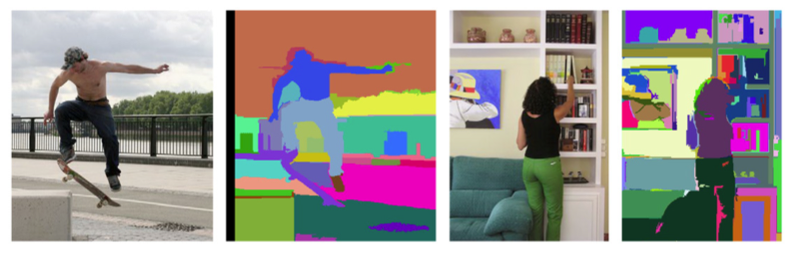
\includegraphics[width=15cm]{imgs/ch2/segment}
\caption{基于图的图像分割结果}
\label{fig:segment}
\end{figure}

%%%%----------------------------------------融合--------------------------------------------%%%%
\section{图像融合}

图像融合是指将多幅包含相关信息的图像处理成一幅图像的过程。相比于每一幅输入图像,输出图像往往包含了更丰富的信息。图像融合方法大体上可分为两类,一类是空间域融合,另一类是变换域融合。

经过图像配准之后,不同的图像经过2D变换,变换到正确的位置上。对于某些重合区域的像素来说,该位置上有两个或多个以上的像素,图像融合问题就是利用怎样的规则求得这些位置上的像素的值。常见的有取均值法,Brovey方法,主成分分析法以及基于高频率波法,IHS和基于曲波变换等技术。

在本文的图像重建系统中,图像融合是重建部分的最后一步,本文的图像融合有这样几个特点:

\begin{enumerate}
\item 待融合的图像块数很多,通常在几十到几百个;
\item 图像块的大小跨度很大,小的块有几十个像素,大的块有上万个像素;
\item 因为融合之前对每一个图像块进行了分割,所以图像块并不一定是完整的,融合的可能是块的一部分区域;
\item 有一张原图像的下采样图像作为参考图像,为图像融合提供了可靠的依据
\end{enumerate}

通过观察上述四个特点我们发现,如果我们以下采样图像作为第一块拼合图像,采用图像块由大到小的方式依次拼接,那么图像融合的任务转变成逐一将小图像块贴合在一个背景图像上,是一个典型的图像无缝拼接任务,解决这个问题的经典方案是泊松图像编辑。

\subsection{泊松图像编辑}
泊松图像编辑是一种自动的“无缝融合”两张图像的技术,在文献\cite{Perez:2003ul}中首次提出。该方法所用的数学工具是带狄里克雷边界条件的泊松偏微分方程,狄里克雷边界条件指定了在影响域内未知函数的拉普拉斯算子,以及在区域边界上的未知函数值的拉普拉斯算子\cite{张建桥:2010vm}。

算法的构思简洁巧妙。首先定义问题:我们改变的图像是\(S\)(背景图像),我们剪切粘贴的图像是\(g\)(前景)。两幅图像的位置关系如图\ref{poi_dis}所示。

\begin{figure}
\centering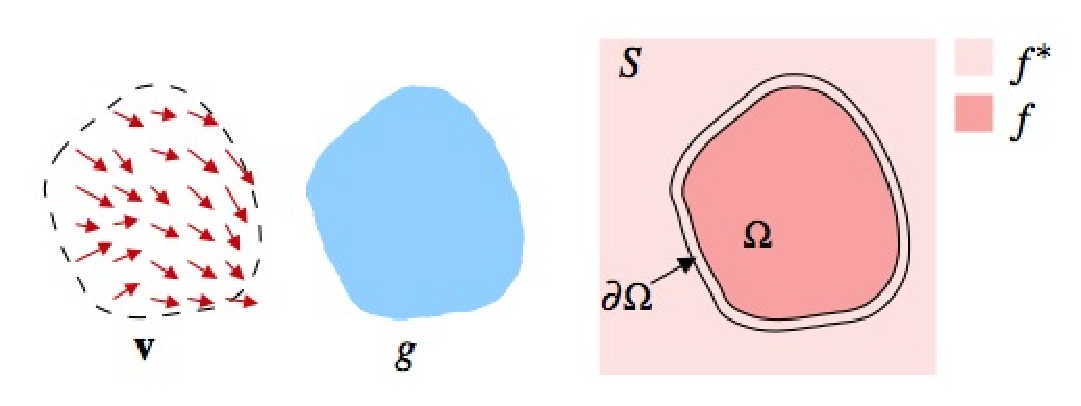
\includegraphics[width=8.00cm]{imgs/ch2/poi_dis}
\caption{泊松图像编辑区域示意图}
\label{fig:poi_dis}
\end{figure}

两幅图像融合的标准时:允许图像B改变颜色,但是仍然能够保留B的完整的“细节”。细节包括B中的边缘、角点、过度等等。而从图像中提取这些细节的多种方法中,都会使用到\textbf{图像梯度}。图像梯度是描述图像的一种数学表达,描述的是像素与相邻像素的相对变化(本质上是像素与其相邻像素的差值)。我们需要寻找的就是相对描述子,因为图像A与图像B之间的不统一主要是因为他们颜色上的绝对差。因此,更为严格的泊松图像编辑的目标是:允许改变绝对信息,即图像B的颜色,但是在粘贴之后尽可能的保留B的相对信息,即图像梯度。

我们将图像B的边缘像素固定,其像素值为图像A的像素值,然后求解其余的在选取内的像素值,约束条件是保持图像B的原始梯度。

设对g进行校正后得到的图像是f,f能够更好的与S融合。g的边界与S的边界完全一致,匹配选取内部的像素,向内融合:

\begin{equation}
f_{(x,y)} = S_{(x,y)}\forall{(x,y)}\in{\partial{f^*}}
\end{equation}
其中\(\partial{f^*}\)表示\(f^*\)的边界

我们期望H内部像素的梯度值等于B内部像素的梯度值。一个点上图像梯度的定义是:该像素与所有像素的差值的和
\begin{equation}
|\nabla{f^*_{(x,y)}}| = 4f^*(x,y) - f^*(x-1,y) - f^*(x+1,y) - f^*(x,y-1) - f^*(x,y+1)
\end{equation}

我们需要解决的问题是一个求最小值的问题:
\begin{equation}
\mathop {min}\limits_{f}\iint_{\Omega}^{} |\nabla{f}|^2\text{ with }f|_{\partial\Omega} = f^*|_{\partial\Omega}
\label{fusion_problem}
\end{equation}
这个求最小的问题满足欧拉-拉格朗日(Euler-Lagrange)等式:
\begin{equation}
\Delta f = 0\text{ over }\Omega\text{ with }f|_\partial{\Omega} = f^*|_\partial{\Omega}
\label{eul-lag}
\end{equation}

其中\(\Delta = \frac{\partial^2.}{\partial{x^2}}+\frac{\partial^2.}{\partial{y^2}}\)是拉普拉斯算子,公式\eqref{eul-lag}是满足Dirichlet边界条件的拉普拉斯等式。
我们将公式\eqref{fusion_problem}稍加修改,引入一个引导域\(v\),得到如下结果:
\begin{equation}
\mathop {min}\limits_{f}\iint_{\Omega}^{} |\nabla{f} - v|^2\text{ with }f|_{\partial\Omega} = f^*|_{\partial\Omega}
\label{fusion_problem2}
\end{equation}

公式\eqref{fusion_problem2}的解是满足狄利克雷边界条件的泊松等式:
\begin{equation}
\Delta f = div\mathbf{v}\text{ over }\Omega\text{ with }f|\partial{\Omega} = f^*|\partial{\Omega}
\label{poi_equ}
\end{equation}
其中\(div\mathbf{v} = \frac{\partial u}{\partial x}+\frac{\partial v}{\partial y}\)是\(\mathbf{v} = (u,v)\)的散度。

上式等效于求
\begin{equation}
\Delta \tilde{f} = 0\text{ over }\Omega,\tilde{f}|\partial{\Omega} = (f^* - g)|\partial{\Omega}
\label{poi_equ}
\end{equation}

其中\(f = g + \tilde{f}\),我们的问题转变成求差值的问题。

\subsection{泊松图像编辑离散解}
如果一个相邻像素是(1)边界像素,那么它的值是固定的;(2)超出选区边界,被排除。下面的差分方程总结了每一个像素点的所有情况
\begin{equation}
\begin{aligned}
|N|f(x,y) - \mathop {\Sigma }\limits_{(dx,dy)+(x,y) \in{\Omega}}f(x+dx,y+dy)
-\mathop {\Sigma }\limits_{(dx,dy)+(x,y) \in{\partial{\Omega}}}A(x+dx,y+dy) \\
= \mathop {\Sigma }\limits_{(dx,dy)+(x,y) \in{\Omega \bigcup {\partial{\Omega}}}}
f^*(x+dx,y+dy) - f^*(x,y)
\end{aligned}
\end{equation}

其中\((x,y)\)是2D网格上感兴趣的像素点的位置。N是相邻像素的数量(包含边界像素,N<=4)。\(\Omega\)是B选区(不包含边界),\(\partial \Omega\) 是边界,\((dx, dy)\)是可能的相邻像素点位置,包括 {(-1, 0), (1, 0), (0, -1), (0, 1)}。

等式左侧是计算未知像素点\(f(x, y)\)的空间梯度,计算的方式是将\(f(x,y)\)与每一个相邻的像素点做差值,并加和。每一个差值的形式都是\(f(x,y) - other(x',y')\),其中\((x',y')\)是其他像素点的位置。

等式右侧计算\(f^*\)图像在(x,y)处的梯度值,它与我们新的图像\(f\)的像素值匹配。

对于RGB图像,这些公式会分别处理R,G,B三个通道。

下一步我们需要为H中的每一个点列出等式,注意到我们列出了一组线性方程,包含k个未知数,k是我们需要求解的H中像素数量,最直接的方案是把所有的方程放到一个矩阵中,然后反转矩阵。然而,k的值相当的大,对于200X200的选取而言,k是40,000。反转一个40000X40000的矩阵太庞大了。我们注意到矩阵是极为稀疏的,因为每一个点至多有4个相邻像素,(并且是正定的)。每一行至多有5个非零的元素,其余是0。针对这样的特性,可以采用迭代矩阵求解算法。为了简便,我决定使用 Jacobi Method来求解稀疏线性方程组。Jacobi Method是梯度下降算法的一个特例。它的基本思路是:

\begin{itemize}
\item 以\(A x = b\) 的形式建立矩阵等式。A是我上述定义的等式的矩阵,x是我们待求解的值(本例中是H图像的像素值),b是等式需要等于的值。如果你有一个稀疏矩阵,对它进行压缩是一个好主意(我的程序仅仅用数据结构存储哪些非零的条目);
\item 初始化x,使之全为0;
\item 计算\(Ax\)的积;
\item 计算\(b-Ax\)的差值,这个差值衡量的是当前猜测的x的值和正确值之间的误差;
\item 将差值\((b-Ax)\)追加到x上。这就是我们让猜测向着正确方向前进的“梯度下降”的步骤;
\item 重复步骤3-5,直到x和\((b-Ax)\)之间的差值足够小;
\end{itemize}

因为A是正定的,这个过程能够保证收敛到x的正确的解,并以指数速度收敛。

\subsection{卷积近似解法}
解等式\eqref{poi_equ}需要多次迭代,耗费大量时间,文献\cite{Farbman:2011dc}使用薄膜插值法(Membrane Interpolation)。\(f^*\)的值可以通过近似方法得到,其思路是沿着区域边界平滑的拓展差值,直到展开到整个区域。差值可以写成卷积的形式:
\begin{equation}
\tilde{f} = \frac{G * \tilde{r}}{G * \tilde{R}}
\label{con_pyr}
\end{equation}
其中
\begin{equation}
\begin{cases} 
\tilde{r}(x_i) = f^*(x_i) - g(x_i), & \forall{x_i} \in \partial\Omega \\
0, & \mbox{其它}
\end{cases}
\label{con_pyr}
\end{equation}
而\(\tilde{R}\)是\(\tilde{r}\)的特征函数,\(G(x_i,x_j)\)是平移不变格林函数:
\begin{equation}
G(x_i,x_j) = G(\|x_i - x_j\|) = 2\pi\log{\frac{1}{\|x_i - x_j\|}}
\end{equation}
卷积可以通过三个个滤波器进行快速的计算,这个计算的时间复杂度是O(n),与像素数量呈线性关系。实验表明采用卷积近似解泊松方程得到的解的像素值和采用迭代求解差异不大,适用于本文的图像融合的场景下。


%% 本章参考文献
\ifx\usechapbib\empty
\nocite{BSTcontrol}
\bibliographystyle{buptgraduatethesis}
\bibliography{bare_thesis}
\fi
%%
%% 第三章
%% 2012.5.22


\chapter{大规模近似重复图像搜索算法}

随着多媒体业务的日益增长,近似重复图像搜索(Near Duplicate Image Retrieval)或部分重复图像搜索(Partial Duplicate Image Retrieval)技术得到了愈加广泛的应用。在我们的图像重建系统中的相似图像搜索环节,我们希望找到尽可能多的与用户拍摄图像相似的图像,将其作为后续重建环节的候选图像。因此我们面临的三个技术难点是:(1)相似搜索是在图像的局部进行的,而不是整幅图像,所以使用全局特征进行相似图像搜索的传统方案并不适用,是否有能表述局部特性的图像表示方法;(2)图像的局部特征信息较少,如何充分利用特征之间的几何位置关系进行图像局部匹配来提高搜索精度;(3)云端图像数据库是Web规模的(Web-Scale),图像数据量极大,对算法的时空复杂度限制较大。如何在使用图像局部特征和其空间位置关系的同时尽量不增加搜索算法的复杂度,是本系统需要解决的难题。

本章首先介绍传统的图像搜索算法,再介绍利用局部空间信息生成视觉词组进行相似图像搜索算法,对视觉词组的编码做了进一步的优化。

%%%%----------------------------------------相似图像搜索--------------------------------------------%%%%
\section{基于视觉词袋模型的图像搜索算法}

基于视觉词袋模型的图像搜索算法包含两个环节。第一步,从图像中提取局部特征,图像的感兴趣区域可以通过自动的特征点检测或者均匀取样获得,最常见的局部特征描述子包括梯度方向直方图(histograms of oriented gradient,HOG)和SIFT、SURF等。从一幅图像抽取的特征集合叫做视觉词袋(Bag of Visual Words)。第二步,我们需要定义两个视觉词袋之间的相似性,第一类是直接比较两个视觉词袋的相似性,例如投票方法;第二类是通过视觉词袋计算一个特征签名(signature,通常是一个向量),进而比较两个签名之间的相似度。两种方式都需要对数据库中的所有图像与请求的图像比较相似度并排序\cite{POLICY:2013te}。

\subsection{视觉词袋模型}
视觉词袋(Bag of Visual Words)模型是图像表示中最为经典的一种表示方法。它经常被用来进行图像分类和相似性搜索领域。它来自文档检索基于关键字查询的方法中词袋(Bag of Words)的表示方法,其基本思想是:(1)统计语料库中的所有单词,生成单词表;(2)对于每一篇文档,统计每一个单词出现的频次,用由这些单词出现的次数生成直方图,用直方图来表示这篇文档。这种直方图的表示就是词袋表示。视觉词袋类似于BoW模型,算法的基本思路如下:

(1)离线部分:
\begin{itemize}
\item 提取特征:根据使用场景与实际业务的不同,可以选择不同的特征,文献\cite{Zhang:2006ej}对视觉词袋模型进行深入的分析,综合比较了各种特征检测器、描述子等。在这一步,我们综合考虑特征的时空复杂度、鲁棒性、可区分性等。
\item 生成视觉词码表:统计图像数据库中出现的所有特征,去除冗余的特征(比如几乎每一篇文档中都会出现的特征,类似于文档中的停用词)组成视觉词码表(Codebook)。如果提取的图像特征过多,一般需要对特征进行量化,利用聚类算法先把相近的单词归为一类(类似于文档检索里的找词根),利用聚类的结果生成视觉词码表。
\item 利用视觉词码表量化所有的图像特征
\item 利用词频表示的词袋模型来表示数据库中的每一幅图像
\end{itemize}

(2)在线部分:
\begin{itemize}
\item 提取请求图像的局部特征;
\item 利用视觉词码表量化该图像的图像特征;
\item 利用词频表示的词袋模型来表示请求图像;
\item 利用词频表示做进一步的处理,例如分类,相似性比较等。
\end{itemize}

%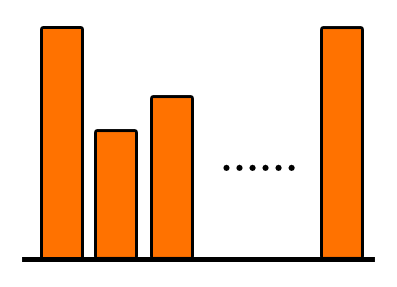
\includegraphics[width=5.00cm]{imgs/ch3/histogram}

\subsection{局部特征的聚类}
生成视觉词码表是将局部特征进行聚类的过程,最经典的聚类算法是K均值聚类(K-MEANS),在实际中,我们通常在云端图像语料集中随机的选取一部分的特征,对这部分特征使用K-MEANS进行聚类,确定所有类中心后,再对语料集中的所有特征进行处理,找到每一个特征距离最近的类中心,完成对所有局部特征的量化。后续的请求图像在提取特征后按照同样的方式进行量化。

然而,在本文提出的系统中,图像局部特征数量极大(对于上百万图像素的图像来说,每幅图像的sift数量平均在3000以上,100K的图像集上,有300M以上个128D的特征),传统的K-MEANS不能满足我们的性能要求,最近的一些研究针对图像据图特征提出了许多快速聚类的方法,文献\cite{Philbin:2007fk,Muja:2009uv,Wang:2010vs}等提出了近似K聚类(Approximate K-MEANS,AKM)和结构化K聚类(Hierarchy K-MEANS,HKM)的方案。

近似K-MEANS是传统K-MEANS的一种替代,传统的K-MEANS的时间花销主要是在计算特征点最近邻的类中心上,每一次迭代,我们需要计算每一个特征点,计算它和每一个类中心的距离,所以每次迭代的时间复杂度是\(O(NK)\),其中N是特征点数量,K是类中心的数量。在改进的版本中,每一次迭代之前,我们使用随机k-d森林来构建类中心来加快速度。在常规的k-d树中,我们需要决定每一次划分是在哪一个维的哪一个点上,通常我们选择方差最大的一个维度作为划分维度,以该维度上中值点作为划分点,在同一维度上比划分点小的点落在k-d数当前节点的左侧,大的落在右侧。在随机k-d森林中,每一棵k-d树都是构建在所有的类中心上,不过在构建时采用划分策略有所不同,划分维度是方差较大的几个维度中随机选择的,划分点也是随机的在中值附近选择一个点。所有的k-d树组成了k-d森林,这个森林构建了一个互相交叠的特征划分空间。因为量化的存在,一个在划分边缘的特征很可能找到错误的最近邻类中心,而互相交叠的划分方式则大大减轻了这一影响,增强了高维计算的鲁棒性。

计算一个特征点所属类的过程如下:
对随机森林中的每一棵树,递归的下滤到其叶子节点,计算它到可区分边界的距离,将所有的距离记录在一个优先队列中。迭代的选择最近的划分,持续的将隐藏节点加入到优先级队列中,当迭代次数达到指定数值的时候,搜索停止。

K-MEANS的时间复杂度是\(O(NK+N) = O(NK)\),AKM算法的时间复杂度是\(O(Nlog(K)\)。实验表明,AKM在大幅降低时间复杂度的同时,保证了正确率(与K-MEANS划分的类中中心相比不一致的几率小于百分之一)。

%--------------------------------------TO Do Here---------------------------%

\subsection{K近邻算法与相似性度量}
确定空间中某个实例所属的类这一分类问题最常用的解决方案是K近邻算法。
K近邻算法(K-Nearest Neighbor algorithm,KNN)是给定一个训练数据集,对新的输入实例,在训练数据集中找到与该实例最邻近的K个实例,这K个实例的多数属于某个类,就把该输入实例分类到这个类中。

如何找到邻居,邻居的判定标准是什么,用什么来度量是本章节探讨的主要问题。特征空间中两个实例点的距离和反应出两个实例点之间的相似性程度。K近邻模型的特征空间一般是n维实数向量空间,使用的距离可以使欧式距离、曼哈顿距离、标准化欧氏距离、汉明距离、夹角余弦等,由于篇幅所限,这里不一一例举。

%[相似度计算](http://blog.sina.com.cn/s/blog_6634c1410100w56x.html)
%http://www.cnblogs.com/v-July-v/archive/2012/11/20/3125419.html

%%%%----------------------------------------改进--------------------------------------------%%%%
\section{改进的相似搜索算法}

随着数据规模的不断扩大,大规模相似搜索算法在近年来快速发展,主要从提高搜索精度以及搜索效率两个方面着手,通过充分挖掘局部特征信息记忆引入外部相关信息扩大搜索词来提升搜索精度,通过局部敏感哈希等算法压缩数据维度,提高搜索效率\cite{POLICY:2013te}。

文献\cite{Li:2013ks}技术,通过视觉显著性(saliency)模型进行比较,消除背景中的噪声。这种方法使得索引和匹配都集中在显著性区域,更能够符合用户的预期。显著值和空间约束都能够被用来进行相似性度量,并且能够高效的进行二级索引,对于大规模的部分相似图像搜索非常有利,但是内存开销比较大。

文献\cite{Negrel:2013ur}描述了目前存在的各种视觉描述子的概况,介绍了相关的索引技术,包括哈希、词袋以及基于树的表示方法。引出内存开销问题并提出一种生成高度压缩签名(highly compact signatures)的方法,包括张量聚合,主成分分析(PCA),基于核的主成分分析(kernel PCA)等一些列算法。它改进了费舍尔向量(Fisher Vector)族 描述子,提高它的可区分性,以及特征签名的大小。

对于相似性视频搜索,它的特点是特征维数特别大,有研究提出了稀疏投影方式进行特征降维,并且使用数据挖掘的知识使用一些元数据(metadata)来共同进行搜索\cite{Wu:2013tb}。使用机器学习技术,学习稀疏投影矩阵(sparse projection matrices)。这种学习方法可以选择性的使用外部信息,比如WikiPedia上的知识和Google搜索结果中的摘要,创建一个语义相关的投影矩阵,生成一个压缩签名,以满足手机媒体检索的诸多限制。手机内存空间小,计算资源有限,传统的将高维特征映射到低维的投影矩阵在手机内存是放不下的。而我们的稀疏投影矩阵是能够在手机上使用的。

下面我们简单介绍各种性能改进的方法。

\subsection{相似哈希与数据压缩}
文本的去重算法中常见的有余弦夹角算法、欧式距离、Jaccard相似度、最长公共子串、编辑距离等,但是只适合于小数据集。

相似哈希(sim-hash)传统的用来判断两篇文章的相似度,将两篇文章映射到低维空间上,并且保持它们互相之间的相似度,但是它很难应用在图像比较上,因为图像的特征是用实数来表示的,尽管可以将其量化,但是两幅相似图像量化后的特征集合交叠的比率仍旧很小,远远小于文档,因为两幅图像不相似的区域的噪声特征非常大。但是如果使用视觉词组,那么如果两个相似区域的视觉词组会非常相同,我们就可以使用simhash了。所以,min-hash的使用场景是特征比较多,相似度比较显著的情况下。

\subsection{最小哈希的相似性比较}
最小哈希方法是一种广泛应用在相似性查找领域的算法。

在生成视觉词带之后,比较两幅图像或者两篇文章的相似度问题转化为比较两个只包含0,1元素的集合的相似度,集合的相似度是Jaccard相似度。
\[JS(A,B)=\frac{|A\cap{B}|}{|A\cup{B}|}\]
我们首先定义一组随机哈希函数\(f_j:\mathcal{V} \to R\),每一个哈希函数是独立的,将一个视觉词映射为一个实数。两个不同的视觉词\(X_a\)和\(X_b\),哈希函数需要满足两点:(1)\(f_j(X_a)\neq f_j(X_b)\);(2)\(P(f_j(X_a)) < (P(f_j(X_b)) = 0.5\)。

注意到函数\(f_j\)能够反映出视觉词集合的一个顺序排列情况,我们定义min-hash就是这个排列中排在最前面的视觉词,因此有
\[m(\mathcal{A}_i,f_j)= arg\mathop {\min }\limits_{X \in A_i}f_j(X)\]
根据上述定义,我们会发现以下这个事实:
\[Pr(m(A,f_j) = (B,f_j)) = \frac{|A\cap{B}|}{|A\cup{B}|} = sim_s(A,B)\]

如果r是随机变量,当\(m(A,f_j) = (B,f_j)\)时值为1,其它情况下值为0的,那么r可认为是J(A,B)的无偏估计。因此我们可以使用min-hash函数将一幅图片或者一篇文章转化为一个数(对该文章中的每一个单词id使用hash函数后得到一个新的id序列,这个序列中的第一个出现1的行号,就是min-hash的值),当我们使用k个hash函数,得到k个值,将原本的高维向量映射到了低维。min-hash在压缩原始集合的情况下,保证了集合的相似度没有被破坏。
文献\cite{Chum:2008jo}中提出将词频-逆文档频率(term frequency–inverse document frequency,简称TF-IDF)融合在传统的min-hash算法中,实验表明能够提高搜索的准确率。

\subsection{局部敏感哈希}
局部敏感哈希(Locality Sensitive Hashing, LSH)通过哈希方法,缩小两两相似(top)计算的范围,或缩小计算中item的维数,从而达到快速计算相似度的方法。使复杂度变为o(nml),其中n为item的量级,m<<n为新的搜索空间,类似于分支限界中的分支,l<<k,类似于降维处理。

使用min-hash对数据降维后,可以使用LSH缩小查找范围,其基本思路是将相似的集合聚集到一起,减小查找范围,避免比较不相似的集合。

对每一列c(即每个集合)我们都计算出了n行min-hash值,我们把这n个值均分成b组,每组包含相邻的r=n/b行。对于每一列,把其每组的r个数都算一个hash值出来,把此列的编号记录到hash值对应的bucket里。如果两列被放到了同一个bucket里,说明它们至少有一组(r个)数的hash值相同,此时可认为它们有较大可能相似度较高(称为一对candidate)。最后在比较时只对落在同一个bucket里的集合两两计算,而不是全部的两两比较。

%%%%----------------------------------------空间信息匹配搜索算法--------------------------------------------%%%%

\section{基于局部相关信息的相似图像搜索算法}

使用视觉词袋模型来表示图像并比较视觉词频向量之间的相似性的方式应用极为广泛,因其建模简单、泛化能力强。但词袋模型忽略了图像包含位置关系这一天然属性,有学者提出利用空间信息进行图像的搜索任务,进一步挖掘图像本身的信息\cite{Philbin:2007fk,Wu:2009bl,Zhou:2010tv,Zhou:2013jz,Xu:2013wc}。值得注意的是,利用图像特征位置关系提升了匹配精度的同时,也加大了算法的复杂度,在实际使用时应根据任务特点选择合适的算法,空间信息在本文的使用是为了进行精确的图像配准和相似图像搜索。

本节将探讨如何利用图像特征点之间的空间位置和尺度相关性来进行更为精确的相似图像搜索,主体的搜索流程如图\ref{fig:similar_flowchar}所示。

\begin{figure}
\centering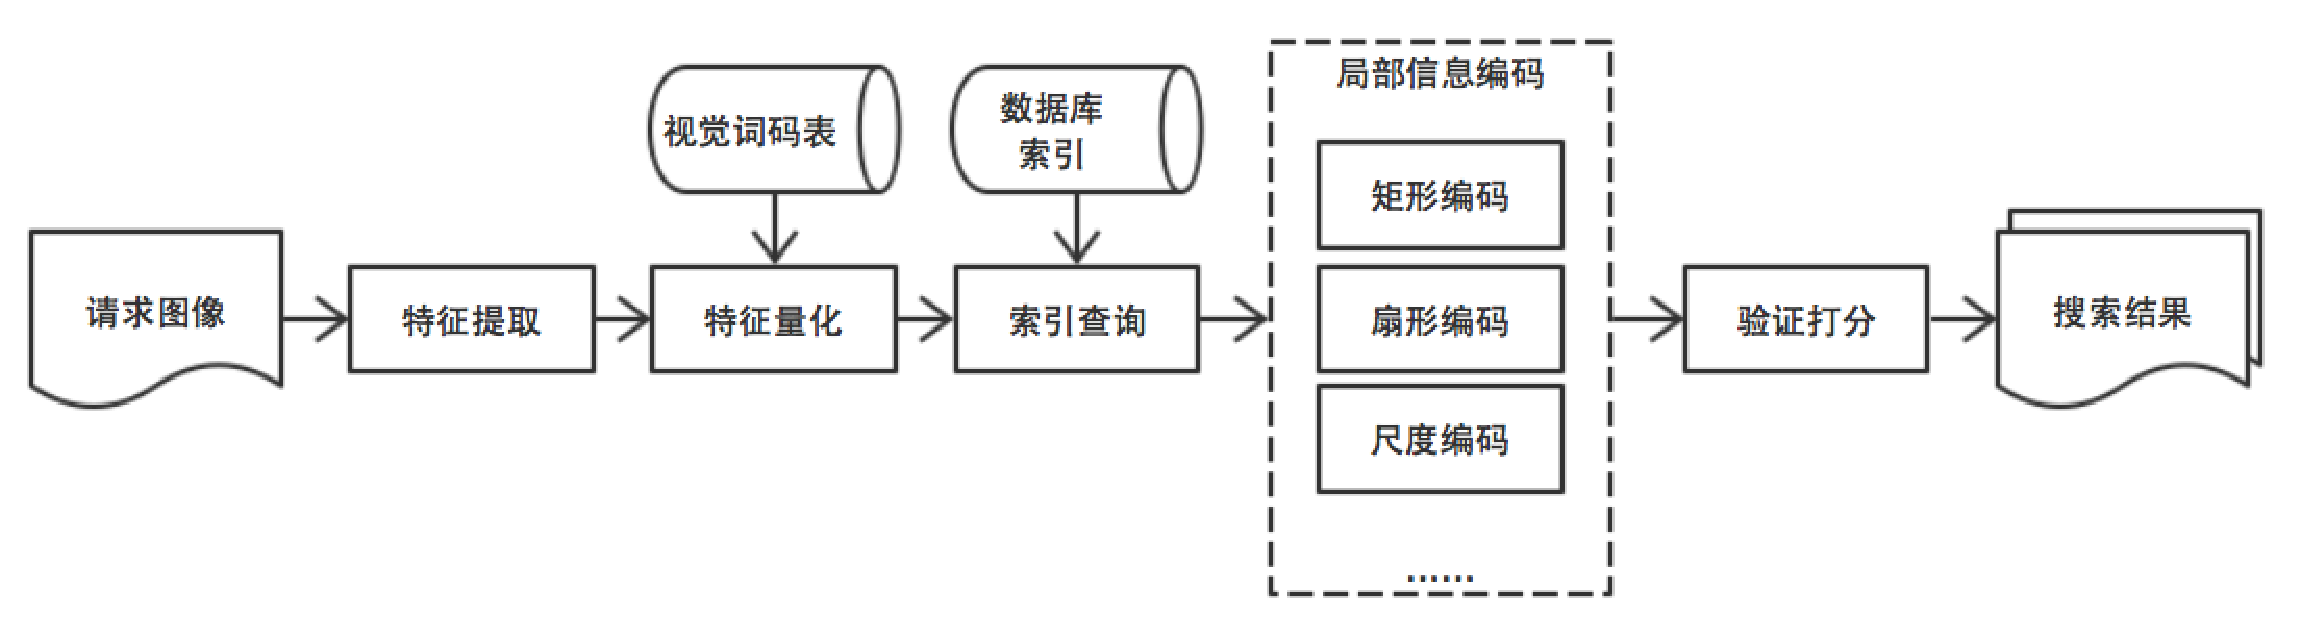
\includegraphics[width=16cm]{imgs/ch3/similar_flowchart}
\caption{利用局部相关信息进行图像搜索流程图}
\label{fig:similar_flowchar}
\end{figure}

其中虚线部分的编码方案有多种方式以及他们之间的多重组合,在实际中应根据应用具体场景采用不同的编码方案。

文献\cite{Xu:2013wc}深入研究SIFT描述子。提出了一个非常优雅的方法:生成SIFT组,嵌入几何信息,最终将一组SIFT压缩到一个64比特的二维签名中,叫做Nested-SIFT。Nested—SIFT使用SIFT描述子的嵌套关系,很自然的将不同尺度的局部关键点组合在一起,生成一个特征签名。嵌入空间信息的Nested—SIFT可区分性更强。使用SimHash进行压缩后,在视觉搜索中效率更高。实验结果表明这种方法提高搜索的准确度,减少了内存消耗,提高搜索速度。其缺点是生成Nested-SIFT会有一定的计算消耗。

文献\cite{Zhou:2013jz}采用较为复杂的空间编码,对图像2D空间进行了不同维度的划分,如图\ref{fig:geo_coding}所示。
\begin{figure}
\centering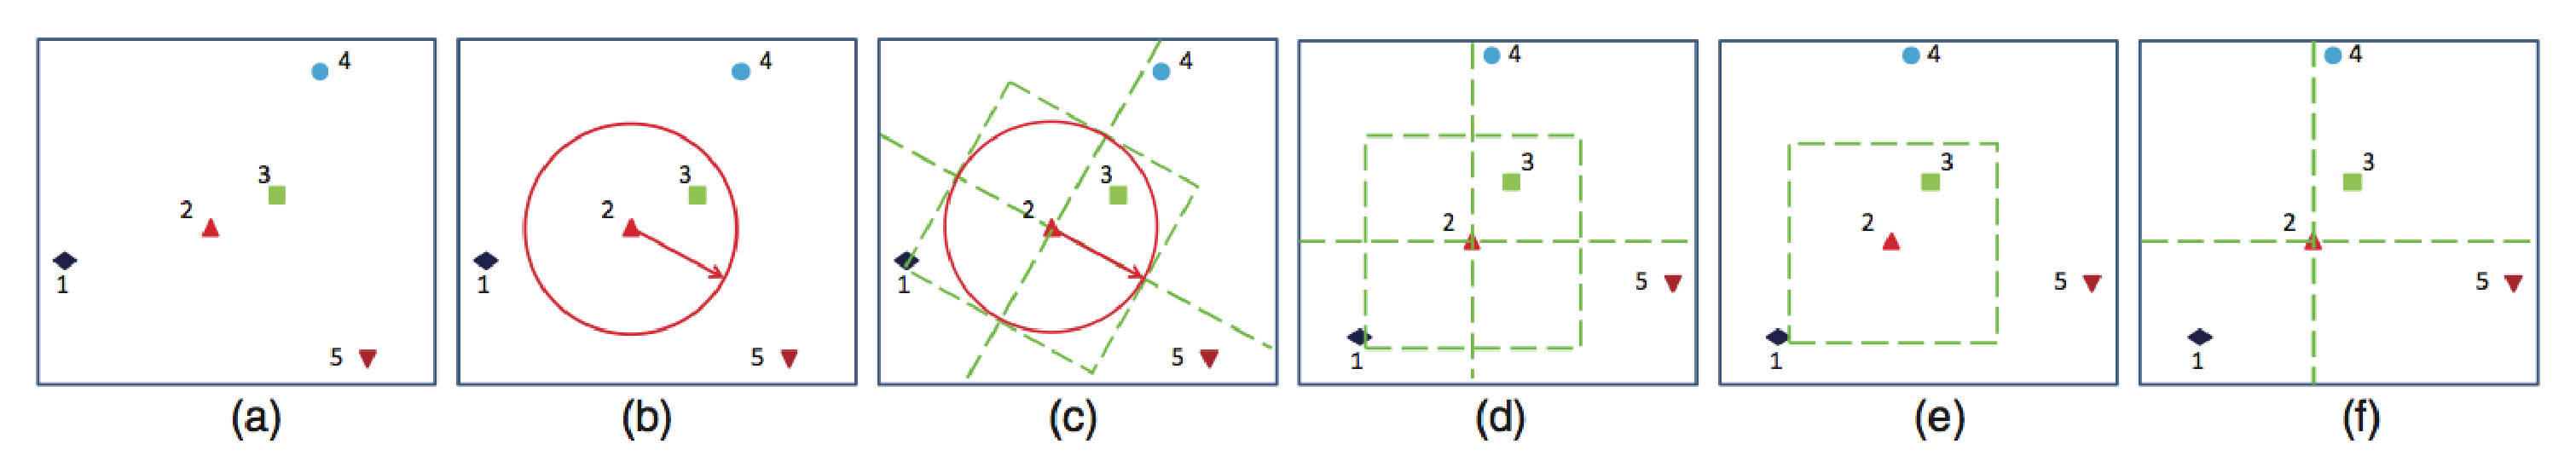
\includegraphics[width=15cm]{imgs/ch3/geo_coding}
\caption{几何编码示例图。(a)图像平面上的五个SIFT特征;(b)红色线条表示编号为2的SIFT特征的尺度、位置和方向;(c)图像平面分区(绿色线条表示);(d)根据c进行旋转后的结果;(e)和(f)表示两种不同的空间划分形式。}
\label{fig:geo_coding}
\end{figure}
首先从正方形区域区分了相邻特征是在区域内还是在区域外图(图\ref{fig:geo_coding}-(e)),其次加入了扇形区域的编码(图\ref{fig:geo_coding}-(f)),增加了视觉词组的旋转不变性。以两种空间划分方式生成编码结果,正如流程图\ref{fig:similar_flowchar}所示,将搜索的中间结果进行空间验证,去除不符合要求的中间结果。

实验结果表明加入空间信息验证后,能够提升准确率,两幅不相关的图像可能会有相似的特征集合,但是相似特征集合在空间位置上依然保持相似的概率极低。但该算法较为复杂,而且编码针对全局SIFT,更加适用于全局图像的相似查询而不适合本文的局部图像块的搜索。

因为本文系统需要查询的是具有局部相似的图像块,相比于其他相似性匹配算法,我们需要的图像块粒度更细,即云端图像与请求图像全局相似度可能很低,但是局部相似度非常高,这幅图像也会被加入到候选图像中。文献\cite{Dai:2012vn}提出了简洁的做法将一个图像块内的局部特征编码成视觉词组。本文在该文基础上做了改进,在保证算法效率的同时,增加了对算子尺度的编码,进一步增强其准确度。

对于每一个图像块而言,中心位置有一个视觉词,该视觉词的尺度与其覆盖范围(影响范围)成正比,在该范围内,有若干视觉词,我们将范围内的所有视觉词看做一个视觉词组(Visual Words Group)。我们希望将词组内的每一个视觉词分配一个编码x,表征这个词在视觉词组的相对关系,这样我们可以采用如下的规则进行匹配:
\begin{equation}
E_m(G_x,G_y) = E_v(G_x,G_y) - E_r(G_x,G_y)
\end{equation}
其中\(E_v(G_x,G_y)\)是能够匹配上的视觉词,这里匹配上定义为两个视觉词相同,并且含有相同的编码x。其中\(E_r(G_x,G_y)\)是错误匹配的视觉词,错误匹配是指两个视觉词相同,但是含有不同的编码x。

那么怎样编码视觉词,能够体现视觉词的相对关系呢?我们从两个维度对视觉词进行编码,一个是它与中心视觉词的相对方向,另一个是相对尺度大小。视觉词组的中心词的主方向作为基准方向,沿着顺时针或者逆时针方向,将整个区域分成n个子区域。接下来对于每一个子区域,根据sift算子量化前的尺度信息对比值大小的不同,将子区域分成r个维度,这样一个视觉词共有n*r个子区域,如图\ref{fig:visual_group}所示。

\begin{figure}
\centering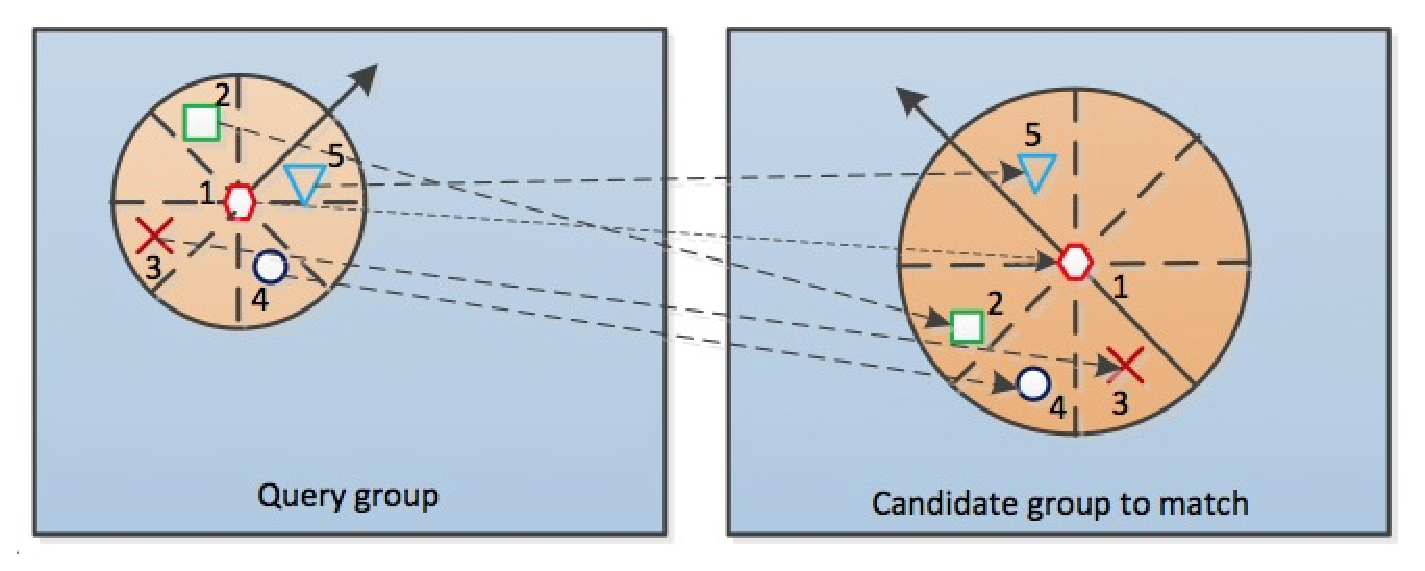
\includegraphics[width=15.00cm]{imgs/ch3/visual_group}
\caption{视觉词组二维编码}
\label{fig:visual_group}
\end{figure}

%%%%------------------------------------适用于旅游景点图像的相似图像搜索技术----------------------------------------%%%%
%\section{适用于旅游景点图像的相似图像搜索技术} 可以不提到

%% 本章参考文献
\ifx\usechapbib\empty
\nocite{BSTcontrol}
\bibliographystyle{buptgraduatethesis}
\bibliography{bare_thesis}
\fi

%% 附录部分

%% 如果有两个或两个以上的附录, 使用appendix环境
\begin{appendix}
  %%
%% This is file `example/app_lhospital.tex',
%% generated with the docstrip utility.
%%
%% The original source files were:
%%
%% install/buptgraduatethesis.dtx  (with options: `app-lhospital')
%% 
%% This file is a part of the example of BUPTGraduateThesis.
%% 

\chapter{不定型($0/0$)极限的计算}
\begin{theorem}[L'Hospital法则]
  若
  \begin{enumerate}
  \item 当 $x \to a$ 时,函数 $f(x)$ 和 $g(x)$ 都趋于零;
  \item 在点 $a$ 某去心邻域内,$f'(x)$ 和 $g'(x)$ 都存在,且 $g'(x)\neq 0$;
  \item $\displaystyle\lim_{x \to a} \dfrac{f'(x)}{g'(x)}$ 存在(或为无穷大),
  \end{enumerate}
  那么
  \begin{align}
    \label{eq:app:lhospital}
    \lim_{x \to a} \frac{f(x)}{g(x)} = \lim_{x \to a} \frac{f'(x)}{g'(x)}.
  \end{align}
\end{theorem}
\begin{proof}
  以下只证明两函数 $f(x)$ 和 $g(x)$ 在 $x = a$ 为光滑函数的情形。
  由于 $f(a) = g(a) = 0$,原极限可以重写为
  \begin{align*}
    \lim_{x \to a} \frac{f(x) - f(a)}{g(x) - g(a)}.
  \end{align*}
  对分子分母同时除以 $(x - a)$,得到
  \begin{align*}
    \lim_{x \to a} \frac{%
      \dfrac{f(x) - f(a)}{x - a}
    }{%
      \dfrac{g(x) - g(a)}{x - a}
    } &
    = \frac{%
      \displaystyle\lim_{x \to a} \frac{f(x) - f(a)}{x - a}
    }{%
      \displaystyle\lim_{x \to a} \frac{g(x) - g(a)}{x - a}
    }.
  \end{align*}
  分子分母各得一差商极限,即函数 $f(x)$ 和 $g(x)$ 分别在 $x = a$ 处的导数
  \begin{align*}
    \lim_{x \to a} \frac{f(x)}{g(x)} &
    = \frac{f'(a)}{g'(a)}.
  \end{align*}
  由光滑函数的导函数必为一光滑函数,故 \eqref{eq:app:lhospital} 得证。
\end{proof}

  % 自动抽取生成缩略语表作为附录A
  \tableofacronyms
  % 用\input{}添加其他的附录
  % \input{...}
\end{appendix}

%% 如果只有一个附录, 使用appendix*环境
%% \begin{appendix*}
%%   % 自动抽取生成缩略语表作为附录A
%%   % \tableofacronyms
%% \end{appendix*}

\ifx\usechapbib\undefined
\bibliographystyle{buptgraduatethesis}
\bibliography{bare_thesis}
\fi

\backmatter
%% 致谢
\ifx\ispeerreview\undefined
%%
%% This is file `example/ackgmt.tex',
%% generated with the docstrip utility.
%%
%% The original source files were:
%%
%% install/buptgraduatethesis.dtx  (with options: `ackgmt')
%% 
%% This file is a part of the example of BUPTGraduateThesis.
%% 

\begin{acknowledgement}
  %% 感谢所有你应该感谢的人
  感谢Donald Ervin Knuth.
\end{acknowledgement}

\fi

%% 在读期间论文发表情况
%%
%% This is file `example/pubs.tex',
%% generated with the docstrip utility.
%%
%% The original source files were:
%%
%% install/buptgraduatethesis.dtx  (with options: `pubs')
%% 
%% This file is a part of the example of BUPTGraduateThesis.
%% 

%% 发表论文列表

%% 攻读学位期间发表论文列表用 tableofpublications 环境产生。需要
%% 在 bare_thesis.tex 的导言区用 \newcite{<name>}{<caption>} 声明不同类
%% 型的论文,具体见导言区说明。
\begin{tableofpublications}
  \thispagestyle{bupt@pubheadings}%
  \bibliographyjrnl{pubs}
  \nocitejrnl{paper1}

  \bibliographyconf{pubs}
  \nociteconf{paper2}
\end{tableofpublications}


\newpage
\end{document}
